\documentclass{article}
\usepackage{graphicx} % Required for inserting images
\usepackage[czech]{babel}
\usepackage{hyperref}
\usepackage{tabularx}
\usepackage{amssymb}
\usepackage{geometry}
 \geometry{
 a4paper,
 total={170mm,257mm},
 left=20mm,
 top=20mm,
 }
 
\newcommand{\modeleq}{\models\!\mid}

\title{Materiály na SZZ pro Informační Bezpečnost}

%připište se kdo upravíte
\author{Matěj Douša}
\date{Červen 2024}






\begin{document}

\maketitle

\tableofcontents

\newpage
\section{Počítače a systémy}
\subsection{SP-19 (PA1)}
Datové typy v programovacích jazycích. Staticky a dynamicky alokované proměnné, spojové seznamy. Modulární programování, procedury a funkce, vstupní a výstupní parametry. Překladač, linker, debugger.

\subsubsection*{Datové typy}
V programovacích jazycích používáme proměnné, tedy něco, co uchovává datovou hodnotu s nějakou vnitřní strukturou. Proměnné jsou identifikovány svými jmény --- identifikátory.
Datový typ proměnné definuje vnitřní strukturu/reprezentaci dat a jejich význam. Tím určuje jakých hodnot může proměnná nabývat a také jaké operace lze s proměnnou (její hodnotou) vykonávat.

\textbf{Jednoduché datové typy:}
\begin{itemize}

	\item celočíselné
	
	\begin{itemize}
		\item existují různé délky --- short, int, long (byte, long long, ...)
		\item signed (znaménkové) --- umí uložit i záporné hodnoty, používá se doplňkový kód
		\item unsigned (neznaménkové) --- ukládá jen kladné hodnoty, přímý kód
	\end{itemize}
	
	\item s pohyblivou řádovou čárkou
	
	\begin{itemize}
		\item existují různé délky --- float, double, long double
		\item znaménko (1 bit) + mantisa (velikost=přesnost) + exponent (velikost=rozsah)
	\end{itemize}
	
	\item znakové
	
		Znaky jsou kódovány jako čísla, používá se ASCII / extended ASCII / UNICODE.
		
	\item logická hodnota
	
		Není v C, ale často se v jazycích vyskytuje (boolean --- true/false).
		
\end{itemize}

\textbf{Další datové typy:}
\begin{itemize}
	\item ukazatel (pointer)
	
		Adresy paměti, kde je uložen datový typ pointeru (pointer vždy ukazuje na konkrétní typ/funkci, případně void).
		
	\item výčtový typ (enum)
	
	\item struktura
	
		Je složena z dalších datových typů, klidně dalších struktur.
		
	\item union
	
		Ukládá více různých datových typů na stejné místo.
		
	\item třída (ve vyšších jazycích)
	
\end{itemize}

\subsubsection*{Statická a dynamická alokace}
Staticky alokované proměnné:
\begin{itemize}
	\item vzniknou běžnou deklarací
	\item ukládají se na zásobník (lokální proměnné) či do části .BSS (neinicializované globální proměnné) a .DATA (inicializované globální proměnné)
	\item v případě pole je nutno znát v době kompilace velikost (statická velikost)
\end{itemize}

Dynamicky alokované proměnné
\begin{itemize}
	\item vzniknou použitím speciální funkcí/operátorem
	\item ukládají se na haldě (heap)
	\item přistupujeme přes pointer
	\item je možné alokovat paměť podle hodnot spočítaných za běhu programu
\end{itemize}

\subsubsection*{Spojové seznamy}
\begin{itemize}
	\item oproti poli nejsou položky seřazeny v paměti, ale každý prvek seznamu obsahuje ukazatel na další prvek.
	\item podobně jako v dynamicky alokovaném poli lze ukládat předem neznámý objem dat
	\item nelze jednoduše indexovat, ale lze libovolně přidávat či ubírat prvky z jakékoliv pozice v seznamu
\end{itemize}

\subsubsection*{Modulární programování}
\begin{itemize}
	\item složitější programy mohou být rozděleny do modulů
	\item tyto moduly lze použít v různých dalších částech programu
	\item modul má svou specifikační část (deklarace poskytovaných prostředků/rozhraní) a implementační část (definice/implementace poskytovaných prostředků)
	\item v C/C++ typicky hlavičkový soubor (.h/.hpp) a implementační soubor (.c/.cpp)
\end{itemize}

\subsubsection*{Procedury, funkce a parametry}
\begin{itemize}
	\item procedura/funkce je posloupnost příkazů uložených v paměti programu
	\begin{itemize}
		\item procedura --- bez návratové hodnoty (typ void)
		\item funkce --- s návratovou hodnotou
	\end{itemize}
	\item použijeme ji zavoláním přes její jméno 
	\item deklarace je specifikace jejího rozhraní --- parametrů a typu návratové hodnoty
	\item definice je samotný kód funkce
	\item vstupní paramtery jsou informace, které využije kód funkce
	\item výstupní parametry jsou výsledkem běhu funkce --- typicky se nějak změní a tím nám dají výsledek
\end{itemize}

\subsubsection*{Překladač}
\begin{itemize}
	\item překládá vyšší programovací jazyky do nižších
	\item ze zdrojového kódu vzniká objektový soubor --- modul se strojovým kódem
	\item front-end přeloží konkrétní jazyk do vnitřní reprezentace (abstrakce nezávislá ani na platformě ani na jazyku)
	\item back-end přeloží vnitřní reprezentaci do strojového kódu konkrétní platformy
\end{itemize}

\subsubsection*{Linker}
\begin{itemize}
	\item spojuje přeložené moduly do výsledného celku --- programu
	\item výstupem je spustitelný soubor
\end{itemize}

\subsubsection*{Debugger}
\begin{itemize}
	\item usnadňuje hledání chyb v kódu, také usnadňuje pochopení programu
	\item je vhodné kompilovat s informacemi pro ladění
	\item je možné si na nějakém místě běh programu zastavit a např. sledovat obsah proměnných, pouštět každý krok programu postupně...
\end{itemize}

\newpage
\subsection{SP-30 (SAP)}
\subsection{SP-28 (SAP)}
Kombinační a sekvenční logické obvody (Mealy, Moore), popis a možnosti implementace na úrovni hradel. Minimalizace vyjádření logické funkce s využitím map.

\subsubsection*{Kombinační obvody}
\begin{itemize}
	\item popsány kombinační funkcí
	\item hodnoty všech výstupů (výstupních proměnných) jsou v každém časovém okamžiku určeny pouze vstupem (hodnotami vstupních proměnných) ve stejném okamžiku
	\item mohou být popsány např. Booleovskou (logickou) formulí
	
	Příklad: $f=x_1.\overline{x_2}+\overline{x_1}.x_2=(x_1+x_2).(\overline{x_1}+\overline{x_2})$
	
	\item obecně kombinační obvod vypadá následovně:
	
	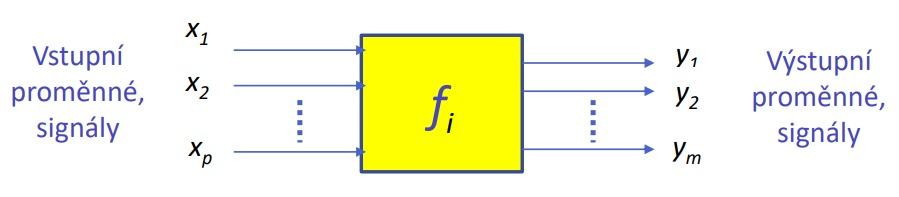
\includegraphics[width=0.7\linewidth]{img/SP-28_0.jpg}
	
	Logická funkce $y_k=f(x_1,x_2,x_3,...,x_p)$	existuje pro každý výstup y.
	
	\item možnosti reprezentace logických funkcí:
	\begin{itemize}
		\item tabulka
		
		\begin{tabular}{ |c|c| }
		\hline
		ab & f \\
		\hline
		00 & 0 \\
		01 & 1 \\
		10 & 1 \\
		11 & 0 \\
		\hline
		\end{tabular}
		
		\item n-rozměrná krychle
		
		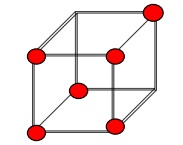
\includegraphics[width=0.2\linewidth]{img/SP-28_1.jpg}		
		
		\item Booleovský výraz
		
		Viz výše		
		
		\item mapa (Karnaughova)
		
		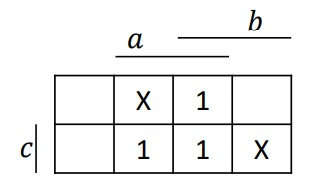
\includegraphics[width=0.25\linewidth]{img/SP-28_2.jpg}		
		
	\end{itemize}
	
	\item možnosti realizace obvodů:
	\begin{itemize}
		\item na úrovni hradel
		\item mapování na technologii (FPGA, ASIC)
		\item popis v jazyku (VHDL, Verilog)
	\end{itemize}
	
\end{itemize}

\subsubsection*{Sekvenční obvody}

\begin{itemize}
	\item výstup závisí na posloupnosti/sekvenci hodnot na vstupu
	\item zapamatování se realizuje zpětnou vazbou
	\item popsány konečným stavovým automatem
	\item typy sekvenčních obvodů:
	\begin{itemize}
		\item Moore
		 
		Obvod, jehož výstup závisí pouze na vnitřním stavu.
		
		\item Mealy
		
		Obvod, jehož výstup závisí také na aktuálním vstupu (kromě stavu).
	\end{itemize}
	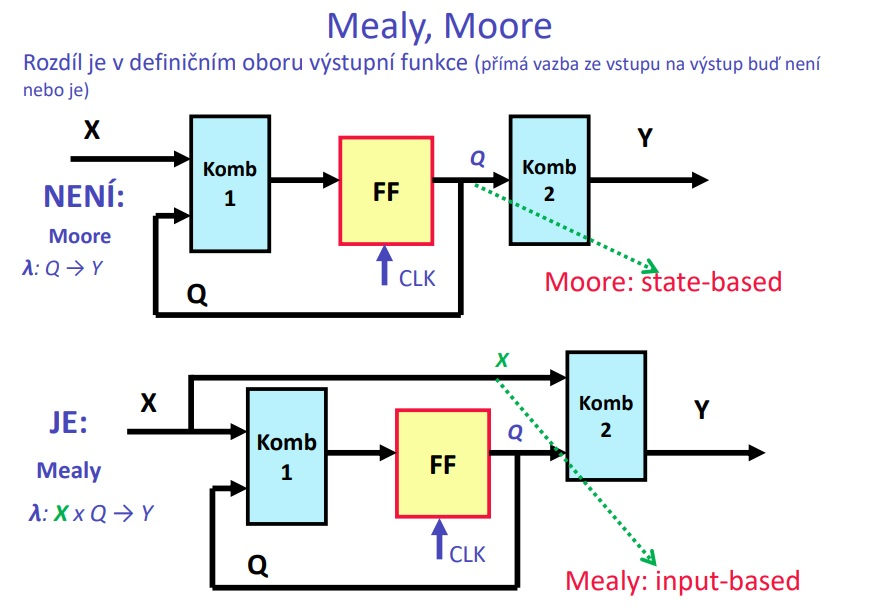
\includegraphics[width=0.6\linewidth]{img/SP-28_3.jpg}		
	
\end{itemize}

\subsubsection*{Implementace na úrovni hradel}
\begin{itemize}
	\item nejprve minimalizace logické funkce a zápis výsledku např. v Booleovském výrazu
	\item následně nakreslení/vytvoření funkce pomocí základních hradel --- NOT, AND, OR, NAND, NOR, XOR
\end{itemize}

\subsubsection*{Minimalizace logické funkce}
\begin{itemize}
	\item smysl --- zjednodušit a zkrátit zápis, snížit potřebný materiál pro výrobu
	\item minimalizace pomocí map --- založenana hledání co největších skupin sousedních stavů.
	\item postup při minimalizaci:
	\begin{itemize}
		\item vytvoření Karnaughovy mapy pro funkci
		\item nalezení všech přímých implikantů (maximální skupiny jedniček či "dont care")
		\item určení všech podstatných implikantů (obsahující jedničku, kterou jiný implikant neobsahuje)
		\item pokud nejsou pokryty všechny vrcholy s "1", nutno vybrat další přímé implikanty (takové, kde je nejméně negací)
	\end{itemize}
	
	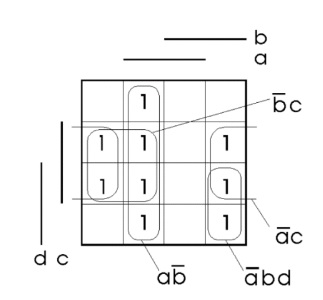
\includegraphics[width=0.4\linewidth]{img/SP-28_4.jpg}
	
	$a\overline{b}+\overline{b}c+\overline{a}c+\overline{a}bd$
	
	\item lze také kroužkovat nuly --- pak je ale nutné funkci sestavit jinak.
	
	$(\overline{a}+\overline{b})(a+c+d)(a+b+c)$
	
\end{itemize}


\subsection{SP-29 (SAP)}
Architektura číslicového počítače, instrukční cyklus počítače, základní třídy souborů instrukcí (ISA). Paměťový subsystém počítače, paměťová hierarchie, skrytá paměť (cache).

\subsubsection*{Architektura číslicového počítače}

\begin{itemize}
	\item architektura se zabývá strukturou a chováním počítače
	
	\item řeší specifikaci různých funkčních modulů jako procesor a paměť a nebo např. instrukční sadu
	
	\item podsměry:
	\begin{itemize}
		\item ISA --- Instruction Set Architecture --- architektura souboru instrukcí
		\item Mikroarchitektura --- konkrétní sestavení a složení procesoru
		\item Systémový design --- řeší další HW komponenty
	\end{itemize}
	
	\item každý počítač je složen z následujících částí:
	\begin{itemize}
		\item datová část procesoru --- ALU, registry
		\item řadič --- řídící jednotka procesoru
		\item paměťový subsystém
		\item vstupní zařízení
		\item výstupní zařízení
	\end{itemize}
	
	\item typy architektury:
	\begin{itemize}
		\item Von Neumannova architektura
		
		Data i instrukce jsou uložena spolu, nejsou explicitně označena/ny.
		
		\item Harvardská architektura
		
		Data a instrukce jsou rozdělené.
	\end{itemize}
\end{itemize}

\subsubsection*{Instrukční cyklus počítače}
\begin{itemize}
	\item čtení instrukce (IF --- Instruction Fetch)
	\item dekódování instrukce (ID --- Instruction Decode)
	\item načtení operandů (OF --- Operand Fetch)
	\item provedení instrukce (IE --- Instruction Execution)
	\item zapsání/uložení výsledku (WB --- Write Back / Result Store)
	\item přerušení?
\end{itemize}

\textbf{Co je instrukce?}
Obsahuje informace:
\begin{itemize}
	\item co se má provést
	\item s čím se to má provést (operandy)
	\item kam se má uložit výsledek
	\item kde se má pokračovat
\end{itemize}

Tyto informace mohou být zadány explicitně, nebo mohou být dány typem instrukce, tedy architekturou počítače --- tedy implicitně.

\paragraph*{ISA --- Architektura souboru instrukcí}

Co je potřeba určit:
\begin{itemize}
	\item typy a formáty instrukcí, instrukční soubor
	\item datové typy, kódování a reprezentace, způsob uložení dat v paměti
	\item módy adresování paměti a přístup do paměti dat a instrukcí
	\item mimořádné stavy
\end{itemize}
Výhody:
\begin{itemize}
	\item abstrakce --- možnost různě implementovat stejnou architekturu instrukcí
	\item definice rozhraní mezi nízkoúrovňovým AW a HW
	\item standardizuje instrukce, bitové vzory strojového jazyka
\end{itemize}

\subsubsection*{Třídy souborů instrukcí (ISA)}
\begin{itemize}
	\item Střadačově (akumulátorově) orientovaná ISA

	Akumulátor je registr pro mezivýpočty, používá se implicitně jako zdroj pro výpočty i jako cíl pro výsledky. Používají se instrukce s jedním operandem. Nejstarší ISA (1949-60) --- vyvinula se z kalkulaček.
	
	\textbf{Výhody:}
	\begin{itemize}
		\item jednoduchý HW
		\item minimální vnitřní stav procesoru --- rychlé přepínání kontextu
		\item krátké instrukce
		\item jednoduché dekódování instrukcí
	\end{itemize}
	
	\textbf{Nevýhody:}
	\begin{itemize}
		\item častá komunikace s pamětí
		\item omezený paralelismus mezi instrukcemi
	\end{itemize}	
	
	Populární v 50. --- 70. letech, HW byl drahý, paměť byla rychlejší než CPU.
	
	\item Zásobníkově orientovaná ISA
	
	Pracovní registry jsou uspořádány do struktury zásobníku.
	Přistupuje se k vrcholu tohoto zásobníku.
	Využití pro vyhodnocení výrazů a vnořená volání podprogramů.
	Většina instrukcí nemá operand (použije se implicitně např. vrchní 2 registry zásobníku).
	
	\textbf{Výhody:}
	\begin{itemize}
		\item jednoduchá a efektivní adresace operandů
		\item krátké instrukce
		\item krátké programy
		\item jednoduché dekódování instrukcí
		\item snadno lze napsat neoptimalizující překladač
	\end{itemize}
	
	\textbf{Nevýhody:}
	\begin{itemize}
		\item nelze náhodně přistupovat k lokálním datům
		\item omezený paralelismus --- zásobník je sekvenční
		\item přístupy do paměti je těžké minimalizovat
	\end{itemize}
	
	\item ISA orientovaná na registry pro všeobecné použití
	
	Dnes převládá. GPR --- General Purpose Registers. Typicky 2 nebo 3 operandy.
	
	\textbf{Výhody:}
	\begin{itemize}
		\item registry (a cache) jsou rychlejší než paměť
		\item k registrům lze přistupovat náhodně
		\item registry mohou obsahovat mezivýsledky a lokální proměnné
		\item méně častý přístup do paměti
	\end{itemize}
	
	\textbf{Nevýhody:}
	\begin{itemize}
		\item složitější překladač (optimalizace pro použití registrů)
		\item přepnutí kontextu trvá déle
	\end{itemize}
\end{itemize}

\subsubsection*{Paměťový subsystém počítače}

\begin{itemize}
	\item cache (skrytá paměť) --- rychlá, drahá, umístěna blíž k procesoru
	\item hlavní paměť --- pomalejší, levnější, větší
	\item vnější paměť --- pomalá, velká
	\item záložní paměť (CD, DVD, flash, magnetické pásky)
\end{itemize}

\begin{itemize}
	\item RAM --- random access memory (přístup adresou)
	\item CAM --- content adressable memory (přístup klíčem)
\end{itemize}

\subsubsection*{Paměťová hierarchie}

\begin{itemize}
	\item registry
	\item L1 cache (SRAM)
	\item L2 cache (SRAM)
	\item L3 cache (SRAM)
	\item hlavní paměť (DRAM)
	\item HDD, SSD
	\item Mass storage (optical disks, tapes)
	\item Remote storage (cloud)
\end{itemize}

\subsubsection*{Cache}

Kopie často používaných dat z hlavní paměti

\begin{itemize}
	\item časová lokalita 
	
	Data, ke kterým bylo právě přistupováno, budou pravděpodobně brzy potřeba znovu.
	
	\item prostorová lokalita
	
	Po přístupu k nějakým datům se pravděpodobně budou používat i vedlejší data.
\end{itemize}
\newpage
\subsection{OB-4 (APS)}
\newpage
\subsection{OB-5 (APS)}
Paměťová hierarchie se skrytou pamětí (cache memory), principy lokality a fungování skryté paměti. Architektura přímé, částečně asociativní, plně asociativní skryté paměti.

\subsubsection*{Paměťová hierarchie}

Rozdíl mezi rychlostí procesoru a rychlostí odpovědi paměti je velký (procesor vs DRAM --- 100x, procesor vs HDD --- 10 milionkrát).
Tento rozdíl se překlene paměťovou hierarchií.

\begin{itemize}
	\item L1 cache
	\begin{itemize}
		\item SRAM
		\item nejmenší, nejblíže jádru, díky tomu nejrychlejší
		\item velikost v řádu jednotek či desítek KB
		\item pro každé jádro zvlášť, bývá rozdělena na instrukční a datovou cache
		\item obsahuje právě nejpoužívanější data a instrukce
	\end{itemize}
	
	\item L2 cache
	\begin{itemize}
		\item SRAM
		\item větší, blízko jádra, latence větší než L1
		\item velikost v řádu stovek KB
		\item pro každé jádro zvlášť, společná pro instrukce a data
		\item obsahuje vše co je v L1 + druhá nejpoužívanější data a instrukce
	\end{itemize}
	
	\item L3 cache
	\begin{itemize}
		\item SRAM
		\item ještě větší, stále poměrně blízko jádrům, latence větší než L2
		\item velikost v řádu jednotek MB
		\item typicky sdílena více jádry, společná pro instrukce i data
		\item obsahuje vše co je v L2 + třetí nejpoužívanější data a instrukce
	\end{itemize}
	
	\item Hlavní paměť
	\begin{itemize}
		\item DRAM
		\item velká, mimo procesor, tedy latence zásadně vyšší než u cache
		\item velikost typicky v řádu jednotek či desítek GB, může být i větší/menší
		\item společná pro celý procesor(y), obsahuje data i instrukce
		\item obsahuje vše co je v L3 + naprostou většinu potřebných dat i instrukcí
	\end{itemize}
	
	\item Sekundární paměť
	\begin{itemize}
		\item HDD, SSD
		\item největší, nejpomalejší
		\item společná pro celý počítač, obsahuje vše
	\end{itemize}
	 
\end{itemize}

\subsubsection*{Principy lokality}
Programy typicky přistupují v daném okamžiku jen k malé části instrukčního a datového adresního prostoru.

\textbf{Časová lokalita:}
\begin{itemize}
	\item položky, ke kterým se přistupovalo nedávno, budou brzy zapotřebí znovu
	\item příklad: opakované procházení dat v cyklu, opakované čtení instrukcí v rekurzivních algoritmech
\end{itemize}

\textbf{Prostorová lokalita:}
\begin{itemize}
	\item položky poblíž právě používaných budou brzy zapotřebí také
	\item příklad: sekvenční přístup k instrukcím programu, sekvenční přístup k datovým polím nebo lokálním proměnným umístěným poblíž sebe
\end{itemize}

\subsubsection*{Principy fungování skryté paměti}
\begin{itemize}
	\item Cache block
	
	Souvislý, nedělitelný úsek hlavní paměti, který lze přenést do cache během jedné paměťové transakce.
	
	\item Cache hit
	
	Úspěšný přístup ke cache block --- tedy úspěšný přístup k datům/instrukcím, které jsou obsaženy v cache a jsou platné.
	
	\item Cache miss
	
	Opak cache hit --- neúspěšný přístup k datům/instrukcím v cache.
	
	\item Hit rate
	
	Úspěšnost přístupů do cache (poměr). 
	
	\item Miss rate
	
	Neúspěšnost přístupů do cache (poměr).
	
	\item Hit time
	
	Latence cache, čas na získání dat z dané úrovně cache.
	
	\item Miss penalty
	
	Celkový čas pro získání dat při výpadku (cache miss) dané úrovně (počítá se od dané úrovně dál).
\end{itemize}

Průměrný čas přístupu do paměti: Hit time + (Miss rate * Miss penalty)

\subsubsection*{Adresace skryté paměti}
Kusy hlavní paměti se do cache ukládají po blocích. Blok může být různě veliký, typicky obsahuje více bytů (nejmenších adreovatelných kusů paměti).


\begin{itemize}
	\item Přímo mapovaná cache
	\begin{itemize}
		\item každý set (řádek) cache obsahuje právě 1 blok.
		\item za sebou jdoucí bloky hlavní paměti se mapují do za sebou jdoucích bloků cache
		\item řádek = (Adresa v hlavní paměti / velikost bloku) \% počet řádků
		\item každý blok hlavní paměti má tedy vždy stejný blok cache kam se uloží.
		\item na stejný blok cache lze uložit více různých bloků paměti, musíme tedy uložit navíc číslo bloku hlavní paměti (část původní adresy) = Tag
	\end{itemize}
	
	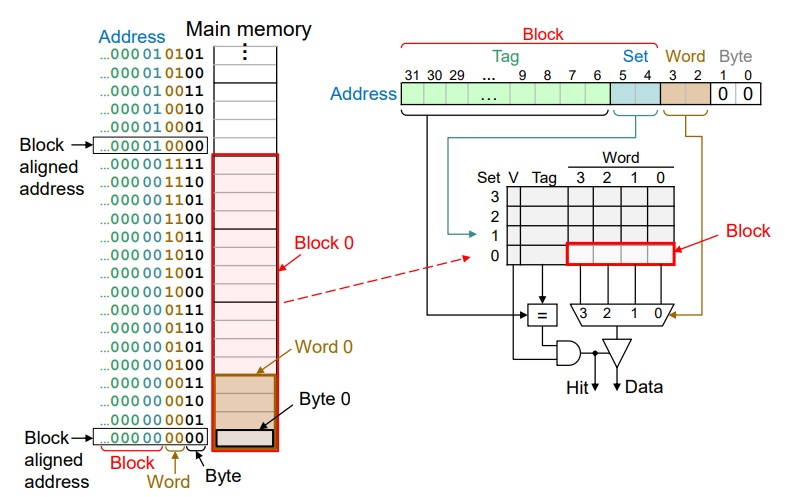
\includegraphics[width=0.8\textwidth]{img/OB-5_0.jpg}
	
	V takovéto cache ale často dochází ke kolizím, když chceme např. přistupovat do více různých částí hlavní paměti. Je ale snazší ji implementovat.
	
	\item Cache s částečným stupněm asociativity
	
	\begin{itemize}
		\item replikace instancí přímo mapované cache
		\item stupeň asociativity je počet takových instancí, neboli také počet cest v cache
		\item bloky hlavní paměti lze uložit na více různých míst (přesně na tolik, kolik je stupeň asociativity)
	\end{itemize}
	
	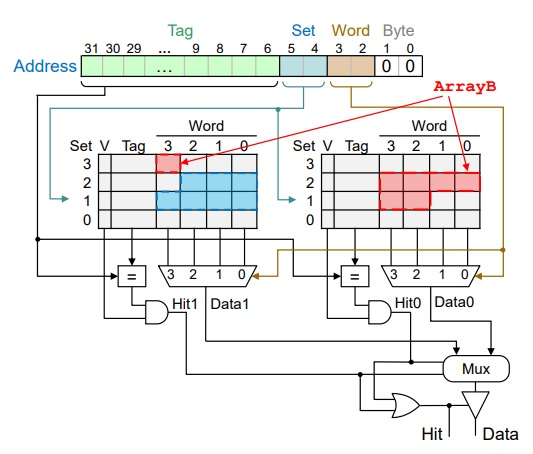
\includegraphics[width=0.7\textwidth]{img/OB-5_1.jpg}
	
	Vyšší složitost implementace, ale zásadně nižší miss rate.
	
	\item Plně asociativní cache
	\begin{itemize}
		\item počet cest je roven počtu bloků cache
		\item instance přímo mapované cache mají tedy jen jeden řádek (set)
		\item u každého bloku se ukládá celá jeho adresa v hlavní paměti
	\end{itemize}
	
	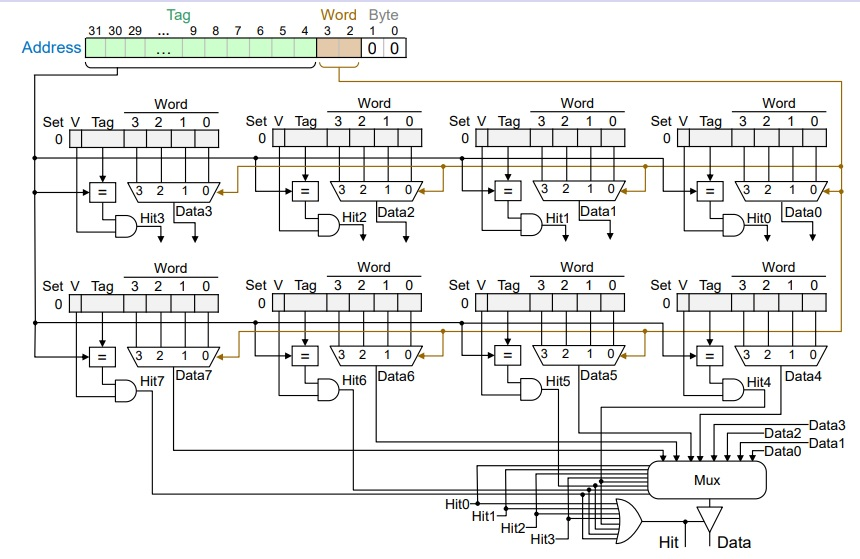
\includegraphics[width=0.75\textwidth]{img/OB-5_2.jpg}
	
	Nejnáročnější na HW prostředky, ale musí řešit maximální počet kolizí.
	
	
\end{itemize}
\subsection{OB-6 (APS)}
\label{OB-6}
HW podpora virtualizace hlavní paměti stránkováním, funkce MMU (Memory Management Unit) a překlad virtuálních adres na fyzické adres pomocí TLB (Translation Lookaside Buffer), ošetření výpadku stránky.

\textbf{Problémy bez virtualizace (motivace pro virtuální paměť):}
\begin{itemize}
	\item Velikost paměti: paměť nemusí být dost velká pro spuštění procesu.
	\item Fragmetace: Při ukončování procesů vzniknou v hlavní paměti volá místa různých velikostí.
	\item Dynamická alokace: Jak alokovat další paměť?
	\item Bezpečnost: Jak zařídit, aby si procesy nemohly číst paměť navzájem?
\end{itemize}

\textbf{Jak funguje stránkování?}
\begin{itemize}
	\item uživatelským procesům je nabídnut Virtuální Adresní Prostor (VAP)
	\item každý proces má svůj VAP
	\item VAP je rozdělen na stejně velké \textit{stránky}, hlavní paměť (HP) je rozdělena nastejně velké \textit{rámce}.
	\item běžící procesy do rámců HP umisťují momentálně potřebné stránky svého VAP (pracovní množina)
	\item nepoužívané stránky se při nedostatku paměti odloží na disk
	\item mapování VAP do HP a přenos stránek mezi HP a diskem zajišťuje OS
	\item virtuální adresa se skládá z čísla stránky a offsetu
	\item fyzická adresa se skládá z čísla rámce a offsetu
\end{itemize}

\textbf{Možnosti překladu virtuálních adres na fyzické:}
\begin{itemize}
	\item Konvenční stránkovací tabulka
	
	Každý proces má svou stránkovací tabulku (většinou strom stránkovacích tabulek).	
	
	\item Inverzní stránkovací tabulka
	
	Všechny procesy sdílejí jedinou, inverzní stránkovací tabulku.
\end{itemize}

\textbf{Jednoúrovňová stránkovací tabulka:}
\begin{itemize}
	\item pro překlad se použije číslo stránky jako index do tabulky, a tam se najde číslo rámce
	\item jednoúrovňová tabulka je ale i pro 32bitové systémy velká, a když ji má každý proces, zabere to hodně místa
\end{itemize}

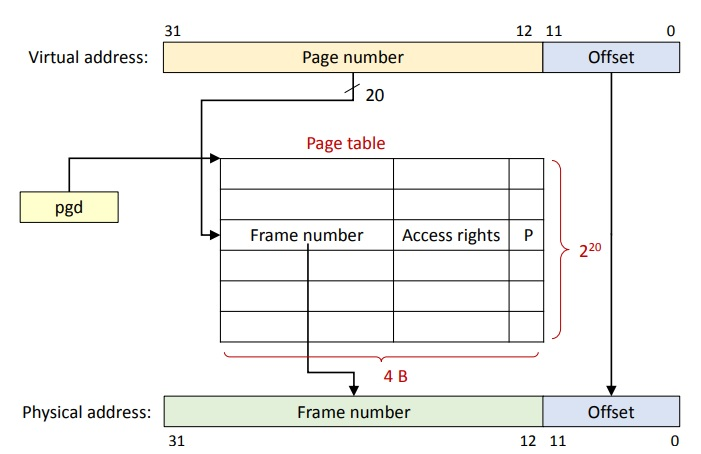
\includegraphics[width=0.8\textwidth]{img/OB-6_0.jpg}

\newpage
\textbf{Víceúrovňové stránkovací tabulky:}
\begin{itemize}
	\item pro překlad se použije číslo stránky, které je složené z indexů do různých úrovní stránkovacích tabulek
	\item jednotlivé tabulky jsou zásadně menší, na počátku stačí jedna tabulka v každé úrovni, další OS může podle potřeby přidat
\end{itemize}

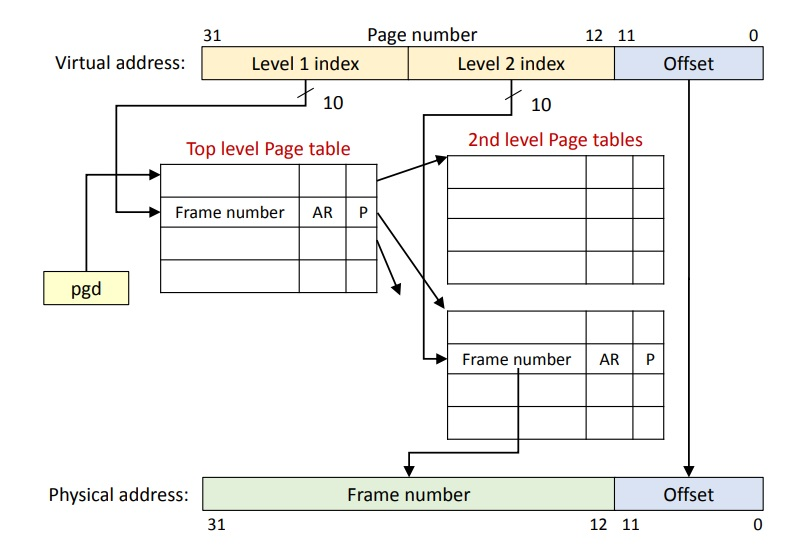
\includegraphics[width=0.8\textwidth]{img/OB-6_1.jpg}

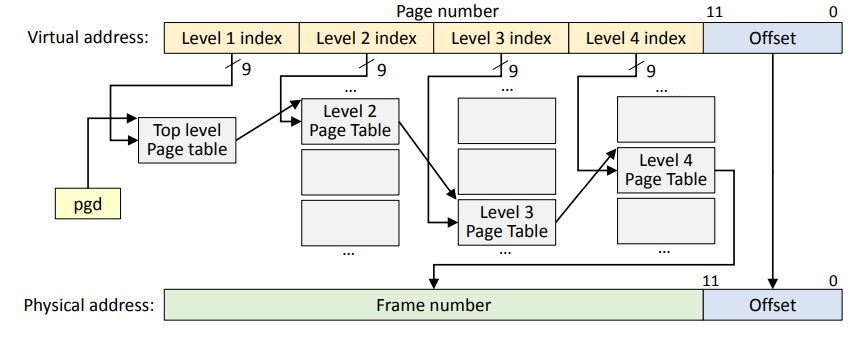
\includegraphics[width=0.8\textwidth]{img/OB-6_2.jpg}

Při překladu VA na FA se musí procházet několik úrovní tabulek stránek (page walk). Ty mohou být uloženy mimo paměť a může dojít k výpadku stránky (page fault).

\subsubsection*{MMU --- Memory Management Unit}
\begin{itemize}
	\item vykonává page walk
	\item dostane adresu stránkovací tabulky první úrovně přes domluvený registr
	\item pokud nedokáže přeložit adresu, nastává page fault, a procesor generuje výjimku
	\begin{itemize}
		\item Invalid page fault --- adresa není součístí adresního prostoru procesu --- obvykle porces zastaven se segmentation fault
		\item Valid page fault --- adresa je součástí VAP, ale nezle přeložit (nenachází se v MMU, tedy musí page walk vykonat OS / překlad neexistuje --- stránka není v HP ale na disku --- OS vymění stránky v HP)
	\end{itemize}
\end{itemize}

\subsubsection*{TLB --- Translation Lookaside Buffer}
Vykonávání page walk je časově náročný proces. Aby nebylo nutné pokaždé page walk vykonávat, každá MMU používá speciální HW překladovou tabulku --- TLB.

TLB jako přímo mapovaná cache:

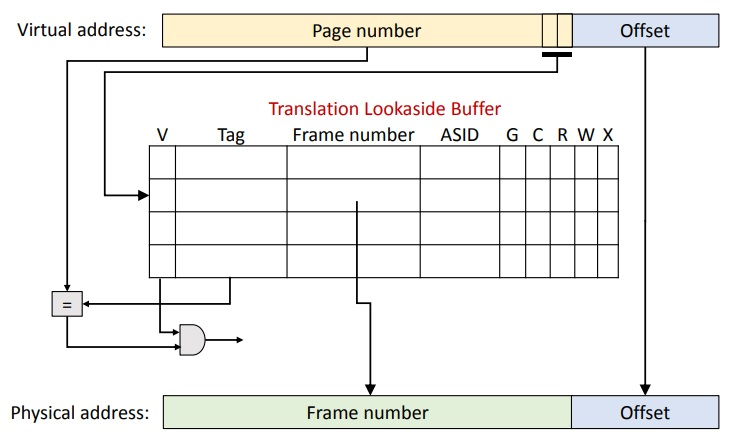
\includegraphics[width=0.8\textwidth]{img/OB-6_3.jpg}

Typicky se používá stupeň asociativity 4-64. Podobně jako u cache se používá SRAM.

Každá položka TLB typicky obsahuje:
\begin{itemize}
	\item V: validity bit
	\item Tag: číslo stránky (část)
	\item Frame number: číslo rámce
	\item ASID: Identifikátor adresního prostoru (pro oddělení procesů)
	\item G: global flag (pokud G = 1, ASID se ignoruje)
	\item C: cache policy (informace, jestli jsou data na adrese "cachovatelná" --- pro I/O zařízení, kam se změny dat musí posílat rovnou)
	\item Access permissions: R, W, X
\end{itemize}

\textbf{Sumarizace HW podpory:}

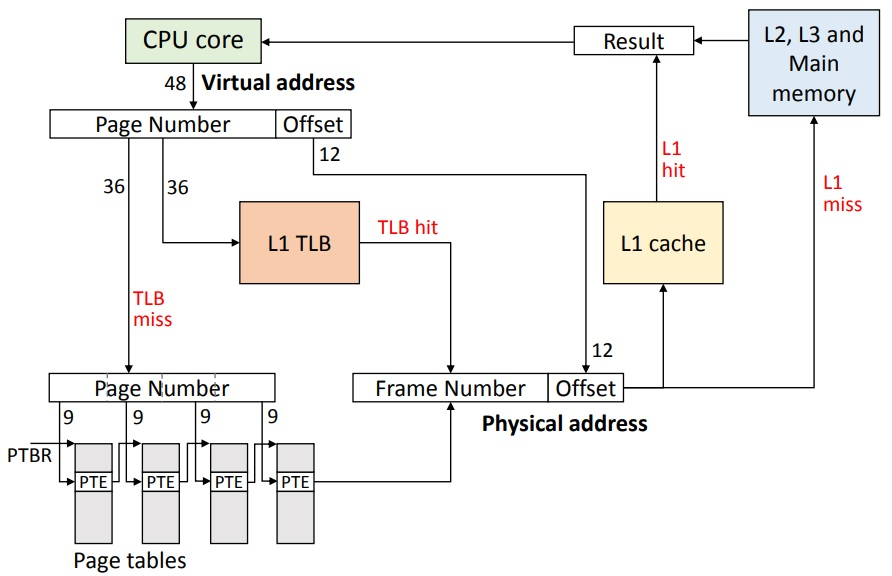
\includegraphics[width=0.8\textwidth]{img/OB-6_4.jpg}
\newpage
\subsection{SP-18 (OSY)}
Virtualizace hlavní paměti stránkováním, principy překladu virtuálních adres na fyzické, struktura tabulek stránek, algoritmy pro nahrazování stránek.

\textbf{Princip virtuální paměti se stránkováním:}
\begin{itemize}
	\item Proces používá virtuální/logické adresy, ty adresují virtuální adresní prostor
	\item VAS (virtual adress space) je rozdělen na stejně velké stránky --- typicky 4KB nebo 8KB
	\item na stejně velké úseky (rámce) je rozdělena fyzická paměť
	\item aktuálně používané stránky musí být aktuálně v hlavní paměti 
	\item virtuální adresa = číslo stránky + offset
\end{itemize}

\textbf{Možnosti překladu adres:}
\begin{itemize}
	\item jednoúrovňová tabulka stránek
	\item víceúrovňová tabulka stránek
	\item invertovaná tabulka stránek
\end{itemize}

Překlad adres zajišťuje MMU s TLB (viz \ref{OB-6}).

\textbf{Jednoúrovňová TS:}
\begin{itemize}
	\item pro každou stránku VAS daného procesu obsahuje jeden řádek obsahující číslo rámce a kontrolní bity (Present bit (P) --- je stránka v hlavní paměti?, Reference bit (R) --- přistupovalo se ke stránce?, Modify bit (M) --- byl obsah modifikován?, Přístupová práva, Cache disabled/enabled, R/W, User/Supervisor (U/S) - lze přistupovat v uživatelském módu?)
	\item číslo stránky = index do této tabulky
	\item pro každý proces jedna tabulka
\end{itemize}

\textbf{Víceúrovňová TS:}
\begin{itemize}
	\item virtuální adresa se skládá z $n$ indexů, které ukazují do tabulek jednotlivých úrovní + offset
	\item tabulky stránek úrovní 1,...,$n-1$ obsahují číslo rámce kde je následující tabulka + present bit
	\item tabulka úrovně $n$ obsahuje present bit + číslo rámce hledané stránky
	\item hlavní/první tabulka je v paměti vždy
\end{itemize}

\textbf{Invertovaná TS:}
\begin{itemize}
	\item obsahuje pro každý rámec fyzické paměti jeden řádek, kde je uloženo: číslo stránky nahrané do rámce, číslo procesu, kterému stránka patří, kontrolní bity, index zřetězení (stejně velký jako index do tabulky)
	\item existuje 1 tabulka pro celý systém
	\item číslo stránky se hashovací funkcí převede na index do tabulky
	\item více stránek se může namapovat na stejný rámec --- proto index zřetězení
\end{itemize}

\newpage
Řešení výpadku stránek:

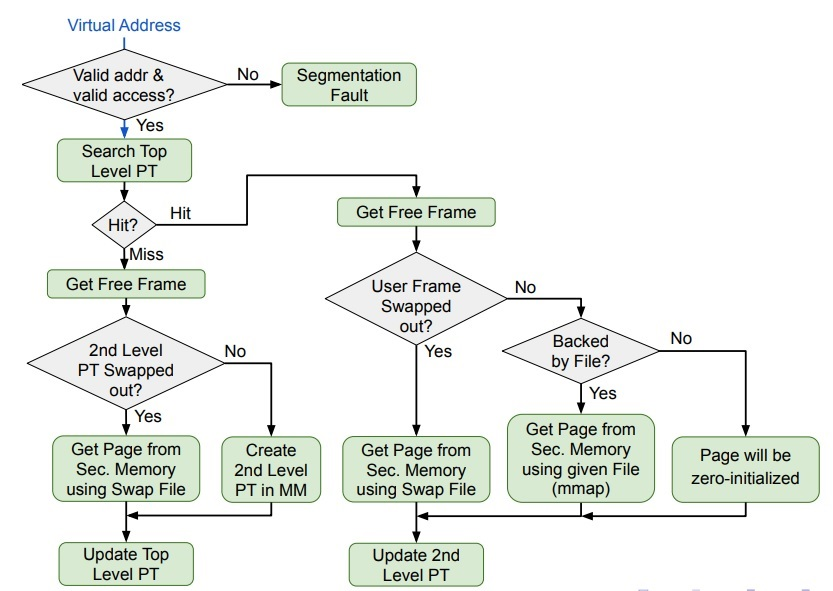
\includegraphics[width=0.6\textwidth]{img/SP-18_0.jpg}
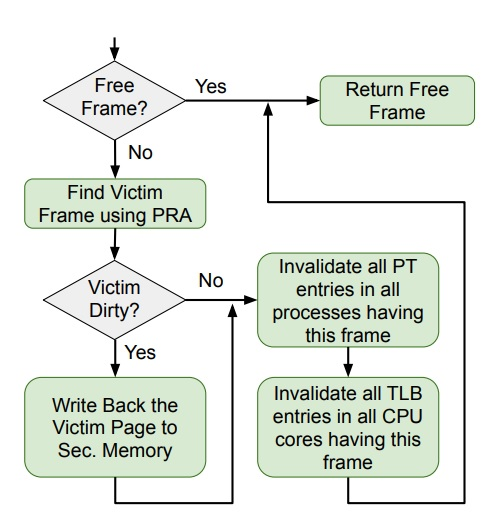
\includegraphics[width=0.35\textwidth]{img/SP-18_1.jpg}

\subsubsection*{Algoritmy pro náhradu stránek}
V okamžiku kdy většina/všechny rámce fyzické (hlavní) paměti jsou obsazené, je úkolem OS najít vhodný rámec, jehož obsah (stránka) se uvolní. K tomu slouží algoritmy pro náhradu stránek.

\textbf{Co je od takových algoritmů požadováno?}
\begin{itemize}
	\item minimalizace počtu výpadků stránek
	\item rychlost
	\item jednoduchá implementace
\end{itemize}

Tyto algoritmy využívají proncipů prostorové a časové lokality.

\textbf{Optimální algoritmus:}
\begin{itemize}
	\item nahradí se stránka, která má čas příštího přístupu nejdelší
	\item generuje minimální počet výpadků stránek
	\item sice nelze udělat, ale slouží pro porovnání kvality reálných algoritmů
\end{itemize}

\textbf{NRU (Not Recently Used)}
\begin{itemize}
	\item pro každou stránku se pamatuje reference bit (R) a modified bit (M) (viz výše)
	\item reference bit se periodicky nastavuje na 0
	\item stránky jsou rozděleny do 4 tříd (RM == 00, RM == 01, RM == 10, RM == 11)
	\item nahradí se nějaká stránka z co nejnižší třídy (tedy 00 $\rightarrow$ 01 $\rightarrow$ 10 $\rightarrow$ 11)
\end{itemize}

Jednoduchý na pochopení i implementaci, poměrně nízký počet výpadků stránek.

\textbf{FIFO (First In First Out)}
\begin{itemize}
	\item je udržován seznam stránek nahraných v paměti
	\item nově nahraná stránka je zaznamenána na konec seznamu
	\item nahrazena je první stránka ze seznamu
\end{itemize}

Jednoduchý na pochopení i implementaci, ale generuje poměrně vysoký počet výpadků stránek.

\textbf{Clock algoritmus}
\begin{itemize}
	\item modifikovaný FIFO algoritmus
	\item seznam stránek jako kruhová fronta
	\item na počátku ručička ukazuje na první položku seznamu
	\item pro každou položku je zaznamenán reference bit, který je nastaven na 1 při pridání stránky do seznamu a při přístupu k ní
	\item při potřebě náhrady stránky ručička u položky, na kterou ukazuje, zjistí stav R bitu --- pokud 1, vynuluje a jde na další položku --- pokud 0, tato stránka se nahradí a ručička se posune
\end{itemize}

Jednoduchý na implementaci, generuje poměrně nízký počet výpadků stránek. Existují varianty s více ručičkami, kde podle rychlosti posunu ručiček a jejich rozevření je definováno časové okno, dle kterého zjišťujeme, zda byla stránka nedávno použita.

\textbf{LRU (Least Recently Used)}
\begin{itemize}
	\item vybere se stránka, která je nejdelší dobu bez přístupu
	\item pro každou položku je navíc zapamatován čas použití, který se aktualizuje při každém použití (existuje globální čítač, který se zvýší při každém přístupu do paměti, jeho hodnota je pak zanesena k právě použité stránce)
	\item kandidát je taková stránka, která má nejnižší čas posledního přístupu (nutno porovnat všechny)
\end{itemize}

Generuje poměrně nízký počet výpadků stránek, dobrá aproximace optimálního algoritmu. Složitější implementace (čítač s časem a porovnání všech stránek)

\textbf{Aging algoritmus}
\begin{itemize}
	\item simulace LRU lgoritmu
	\item pro každou stránku je zapamatováno: R bit (nastaví se na 1 při každém přístupu), $n$-bitový čítač \textit{C}, který má po načtení stránky do paměti všechny bity na 1
	\item periodicky se pro každou stránku \textit{C} posune o 1 doprava, jeho nejvýznamější bit se nastaví na R, a R se nastaví na 0
	\item vhodným kandidátem je stránka s nejnižší hodnotou \textit{C}
\end{itemize}

Menší režie než LRU, ale není tak přesný (nepamatuje se přesný čas, ale jen interval, kdy se naposledy přistupovalo --- omezená historie).
\newpage
\subsection{SP-17 (OSY)}
Procesy a vlákna, jejich implementace, nástroje pro synchronizaci vláken. Klasické synchronizační úlohy. Uváz\-nu\-tí (deadlock) vláken (alokace prostředků, Coffmanovy podmínky, strategie pro řešení uváznutí).

\begin{itemize}
	\item \textbf{Program:} 
	
	Program je v systému reprezentován spustitelným binárním programem, který je uložený v sekundární paměti (např. disk).
	
	\item \textbf{Proces:} 
	
	Instance spuštěného programu/aplikace. Entita, v rámci které jsou alokovány prostředky (paměť, vlákna, otevřené soubory, zámky, semafory, sokety,...).
	
	\item \textbf{Vlákno:} 
	
	Výpočetní entita (proud instrukcí), které je přidělováno jádro CPU. Vlákna vytvořená v rámci procesu sdílí většinu prostředků alokovaných v tomto procesu.
\end{itemize}

\textbf{Vytvoření procesu:}

Nový proces lze vytvořit jako kopii/klon původního procesu, či jako úplně nový proces. V Unixu fork() exec(), ve Windows CreateProcessA().

\begin{itemize}
	\item \textbf{fork():}
	
	Vytvoří nový proces, který je kopií toho procesu, ze kterého byla tato funkce zavolána. V případě chyby vrací -1, v potomkovi vrací 0, v rodiči vrací PID potomka.
	
	\item \textbf{exec():} 
	
	Adresový prostor aktuálního procesu je přepsán obsahem souboru, který se začne vykonávat od začátku.
	
	\item \textbf{wait():} 
	
	Zablokuje rodičovský proces, ve kterém je zavolána, dokud se konkrétní/jeden potomek neukončí.
\end{itemize}

\textbf{Ukončení procesu:}
\begin{itemize}
	\item jádro se pokusí předat návratový kód rodiči
	\item ukončí se všechna vlákna pod procesem
	\item uvolní se adresový prostor procesu a příslušné struktury OS
	\item proces se může ukončit sám (buď normální konec programu jako \textit{return}, nebo chyba, kvůli které se sám ukončí), nebo může být ukončen jádrem (fatální chyba nebo signál od jiného procesu)
\end{itemize}

\textbf{Vlákna:}
\begin{itemize}
	\item proces se implicitně vytváří s jedním "main" vláknem
	\item další vlákna lze vytvořit z hlavního (volání OS)
\end{itemize}

\textbf{Plánování:} 
\begin{itemize}
	\item vláken je typicky zásadně více než logických jader procesoru
	\item jedno vlákno je zpracováváno max 1 logickým jádrem
	\item aby se vlákna na jádrech vystřídala, používá se typicky preemptivní plánování
	\begin{itemize}
		\item vlákno je na základě plánovacích kritérií vybráno, a je mu přiděleno volné jádro CPU
		\item vláknu je přiděleno množství času na CPU
		\item vláknu je jádro odebráno, pokud uplyne přidělený čas, vlákno provede systémové volání nebo dojde k přerušení
	\end{itemize}
	\item přepínání kontextu (vystřídání vláken na jádře CPU)
	\begin{itemize}
		\item kontext = všechny nezbytné informace pro pozdější spuštění přerušeného vlákna od okamžiku pře\-ru\-še\-ní
		\item kontext se uloží do paměti, naplánuje se další vlákno a jeho kontext se nahraje do CPU jádra
	\end{itemize}
\end{itemize}

\textbf{Stavy vláken:}

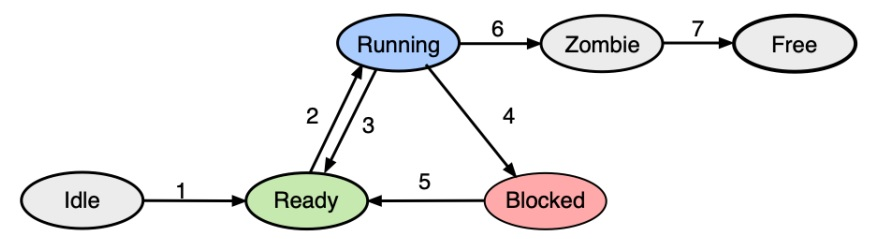
\includegraphics[width=0.8\textwidth]{img/SP-17_0.jpg}

\begin{itemize}
	\item \textbf{Časově závislé chyby:}
	
	Situace, kdy více vláken používá společné sdílené prostředky a výsledek deterministického algoritmu je závislý na rychlosti jednotlivých vláken, které používají tyto prostředky. Špatně se detekují --- lze předcházet správným návrhem paralelního algoritmu.
	
	\item \textbf{Kritická sekce:}
	
	Část programu, kde vlákna používají sdílené prostředky.
	
	\item \textbf{Sdružené kritické sekce:}
	
	Kritické sekce více vláken, které se týkají stejného sdíleného prostředku.
	
	\item \textbf{Vzájemné vyloučení:}
	
	Vláknům není dovoleno sdílet stejný prostředek ve stejném čase, tedy se nenachází ve stejné sdružené sekci současně.
	
	\item \textbf{Korektní paralelní program:}
	
	Nesmí klást předpoklady na rychlost vláken a počet jader. Musí zajistit výlučný přístup ke sdíleným prostředkům. Mimo kritické sekce by vlákno nemělo být zpomalováno ostatními vlákny.
\end{itemize}

\textbf{Problémy s použitím synchronizace vláken:}
\begin{itemize}
	\item deadlock (x vláken čeká na událost, kterou může vyvolat jen jedno z čekajících vláken)
	\item livelock (několik vláken vykonává neužitečný výpočet, ale nemohou dokončit)
	\item starvation (vlákno ve stavu "ready" předbíháno a dlouho se nedostane na řadu)
\end{itemize}

\textbf{Zamykání kritických sekcí:}
\begin{itemize}
	\item zámek značí, zda je ve sdružené kritické sekci už jiné vlákno --- musí se k němu přistupovat atomicky (např. TSL --- Test and Set Lock)
	\item aktivní vs blokující čekání
\end{itemize}

\begin{itemize}
	\item \textbf{Zámek (mutex):}
	
	Pamatuje si svůj stav (zamčený/odemčený) a množinu vláken blokovaných na něm. Jsou nad ním definovány atomické operace lock() a unlock().
	
	\item \textbf{Podmíněná proměnná (conditional variable):}
	
	Pamatuje si, která vlákna jsou na ní blokována. jsou definovány operace cond\_wait(mutex) a cond\_signal(). cond\_wait(mutex) --- mutex musí být zamčen volajícím vláknem, funkce odblokuje mutex a zablokuje vlákno dokud nepřijde cond\_signal().
	
	\item \textbf{Semafor:}
	
	Obsahuje čítač a seznam blokovaných vláken. Jsou definovány operace sem\_init(int) (nastaví čítač na 0), sem\_wait() (vstup do sekce --- pokud čítač je větší než 0 tak vlákno vstoupí a dekrementuje čítač, jinak se zablokuje) a sem\_post() (uvolní nějaké čekající vlákno, nebo inkrementuje čítač).
	
	\item \textbf{Bariéry:}
	
	Obsahuje čítač (síla bariéry --- kolik vláken musí čekat, aby byla odblokována) a blokovaná vlákna. Operace: barrier\_init(int) (nastaví sílu bariéry) a barrier\_wait() (pokud čítač je více než 1, vlákno čeká a čítač je dekrementován, jinak jsou všechna vlákna probuzena)
	
\end{itemize}

\textbf{Synchronizační úlohy:}
\begin{itemize}
	\item Večeřící filosofové
	\begin{itemize}
		\item $N$ filosofů u kulatého stolu
		\item každý má před sebou jídlo a mezi sousedními talíři je vždy 1 vidlička (celkem tedy $N$ vidliček)
		\item pokud chce filosof jíst, musí získat obě vidličky vedle jeho talíře
		\item stavy filosofa: přemýšlí (nechce a nemá vidličky), má hlad (pokouší se získat obě vidličky), jí (má obě vidličky)
		\item optimální řešení: může jíst až $\lfloor N/2 \rfloor$ filosofů, nevznikají časově závislé chyby ani synchronizační problémy
		\item řešení: pokud mam hlad zamknu mutex, kouknu jestli jsou volny vidlicky, pokud ne spim (odemykam mutex), pokud jo, beru, odemykam mutex a jim. Az dojim, zamknu mutex, vratim vidlicky, probudim sousedy a odemknu mutex.
	\end{itemize}
	
	\item Čtenáři --- písaři
	\begin{itemize}
		\item v systému je 1 sdílený prostředek
		\item písaři mohou modifikovat, čtenáři pouze číst
		\item chceme, aby pokud není modifikováno (nepřistupuje písař) mohlo číst více čtenářů
		\item zároveň by nikdo neměl být předbíhán
		\item řešení: písaři i čtenáři se řadí do fronty, ale po skupinách --- pokud přijdu na konec fronty a je tam už stejný typ, přidám se do skupiny --- na začátku fronty je probuzena celá skupina a buď písaři postupně zapíšou, nebo čtenáři společně přečtou
	\end{itemize}
	
	\item Spící holiči
	\begin{itemize}
		\item v holičství je $N$ holičů a křesel k holení, a $M$ křesel k čekání
		\item pokud nejsou zákazníci, holič sedne do holícího křesla a usne
		\item pokud přijde zákazník, buď probudí holiče (pokud je volný), nebo si sedne do čekárny (pokud je místo) jinak odejde
	\end{itemize}
\end{itemize}

\textbf{Obecně alokace prostředku:}
\begin{itemize}
	\item vlákno žádá o prostředek pomocí alokační funkce
	\item pokud je prostředek volný, je přidělen
	\item pokud je již alokovaný, vlákno může být blokováno (v závislosti na alokační funkci --- mutex\_lock blokuje, mutex\_try\_lock blokuje jen na určitý čas, fork() a malloc() neblokují)
	\item v případu 2 a 3 se vlákno pak samo rozhodne jak pokračovat
\end{itemize}

\textbf{Coffmanovy podmínky}

Uváznutí (deadlock) nastane pouze pokud jsou splněny všechny následující podmínky:
\begin{itemize}
	\item Vzájemné vyloučení --- každý prostředek nemůže být sdílen více vlákny
	\item Podmínka neodnímatelnosti --- již přidělený prostředek nemůže být odebrán násilím
	\item Podmínka "drž a čekej" --- vlákno s již přiděleným prostředkem může žádat o další
	\item Podmínka kruhového čekání --- musí existovat smyčka více vláken, ve které každé vlákno čeká na prostředek držený dalším vláknem ve smyčce
\end{itemize}

\textbf{Řešení uváznutí:}
\begin{itemize}
	\item Pštrosí strategie --- ignorování
	\item Prevence uváznutí --- nesplnění alespoň jedné z Coffamnových podmínek
	\item Předcházení vzniku uváznutí --- pečlivá alokace prostředků
	\item Detekce uváznutí a zotavení --- uváznutí je detekováno a odstraněno
\end{itemize}

\textbf{Implementace procesů:}
\begin{itemize}
	\item jádro OS si udržuje zřetězený seznam struktur --- tabulku procesů
	\item jedna položka tabulky obsahuje vše nezbytné, co si OS musí o procesu pamatovat (PCB --- Process Control Block)
	\begin{itemize}
		\item identifikace procesu (id procesu, id rodiče, číslo úlohy/seance/projektu, jméno procesu...)
		\item identita/bezpečnost (vlastník, skupiny, práva procesu)
		\item informace o alokovaných prostředcích (paměť, soubory, prostředky pro meziprocesovou komunikaci)
	\end{itemize}
\end{itemize}

\textbf{Implementace vláken:}
\begin{itemize}
	\item Thread Control Block (TCB) --- identifikace vlákna, info o přepínání kontextu (registry), informace pro plánování vláken
	\item Implementace v uživatelském prostoru (zastaralé)
	\begin{itemize}
		\item OS přistupuje k procesům jako by měly jedno vlákno
		\item proces si svá vlákna spravuje sám
		\item kooperativní plánování pro vlákna v procesu
	\end{itemize}
	\item Implementace v jádře OS
	\begin{itemize}
		\item OS plánuje samotná vlákna, ne procesy
		\item OS udržuje jede PCB pro každý proces, jeden TCB pro každé vlákno
		\item preemptivní plánování pro vlákna v procesu
	\end{itemize}
\end{itemize}

\textbf{Plánování v dnešních OS:} Prioritní Round Robin

$X$ front s různou prioritou. Na základě předchozího běhu vlákna se buď zvýší časové kvantum a sníží priorita (pokud vlákno využilo všechen čas) nebo zvýší priorita a sníží čas (pokud nevyužilo celé časové kvantum).
\newpage
\subsection{OB-3 (ADU)}
\newpage
\subsection{OB-2 (ADU)}
Správa disků a souborových systémů (zařízení, souborové systémy UFS (EXT) a ZFS, disková pole RAID, diskové kvóty), síťové souborové systémy (NFS, CIFS), swap v unixových operačních systémech.
\newpage
\subsection{OB-1 (ADU)}
Identita uživatelů v unixových operačních systémech (identita, práva administrátora, sudo, su, PAM moduly, role, privilegia, identita a přístupová práva, ACL, suid programy).

\textbf{Administrace uživatelů}
\begin{itemize}
	\item konfigurační soubory
	\item uživatelé a jejich primární skupiny v souboru /etc/passwd
	\item hesla uživatelů v /etc/shadow
	\item (sekundární) skupiny uživatelů v /etc/group
	\item přihlašování na jiného uživatele (změna identit): příkaz su [-] [username [argument]] ("-" rozhoduje zda se použijí při\-hla\-šo\-va\-cí skripty cílového uživatele, tedy jestli se změní prostředí)
\end{itemize}

\textbf{Identita procesů}
\begin{itemize}
	\item vnější identita: username, groupname
	\item vnitřní identita: UID, GID
	\item 3 druhy vnitřní identity:
	\begin{itemize}
		\item Reálná (RUID, RGID) --- využívána při akceptaci signálů
		\item Efektivní (EUID, EGID) --- využívána při práci se soubory (vlastnictví, práva,...)
		\item Uložená/saved (SUID, SGID) --- uchování identity při změně EUID/EGID
	\end{itemize}
	\item potomci procesů dědí identity od rodiče, s výjimkou SUID/SGID programů. kdy potomek získá EUID a SUID od vlastníka programu (respektive EGID a SGID) --- např. "su"
\end{itemize}

\textbf{Administrátor}
\begin{itemize}
	\item nazýván root
	\item UID = 0
	\item může všechno --- měnit runlevel systému, vypínat/zapínat systémové služby, používat/přidávat zařízení...
	\item v bezpečnějších systémech pouze jako role --- nelze se přihlásit přímo
\end{itemize}

\textbf{sudo}
\begin{itemize}
	\item \textbf{s}uper \textbf{u}ser \textbf{do}
	\item konfigurace v /etc/sudoers (může měnit jen root)
	\item spuštění konkrétního příkazu jako jiný uživatel (typicky root)
	\item lze nakonfigurovat konkrétní práva pro konkrétní uživatele, lze logovat použití
	\item náchylné k chybám při konfiguraci
	\item běžný účet může díky právům něco zničit
	\item záznam v konfiguraci: who where=(as who) what
	\item možné distribuovat na další zařízení, tedy řídit více systémů
	\item použití většinou vyžaduje heslo aktuálního uživatele (ne toho za koho je příkaz prováděn)
\end{itemize}

\textbf{ACL}
\begin{itemize}
	\item klasická oprávnění (rwx pro vlastníka, skupinu a ostatní) nebyla dostatečná
	\item ACL (Access Control List) jsou dodatečné informace o právech přístupu k souborům (pouze rozšíření, ne náhrada)
	\item umožňují specifikovat rwx práva pro každého konkrétního uživatele a skupinu
	\item lze použít masky
	\item příkaz setfacl a getfacl
	\item není standardem, některé FS/OS neimplementují
\end{itemize}

\textbf{Práva a role}
\begin{itemize}
	\item klasický UNIXový systém řeší práva přes UID (kontroluje, zda UID == 0)
	\item administrátorská práva jsou nedělitelná, problém v případě více administrátorů
	\item systém, který podporuje práva:
	\begin{itemize}
		\item cca 80 práv pokrývajících všechny operace
		\item UID nemá efekt na práva, procesy si s sebou přenáší množinu práv
		\item root má typicky všechna práva, běžný uživatel podmnožinu
		\item 4 množiny práv v procesu: Effective, Inheritable, Permitted, Limit
		
		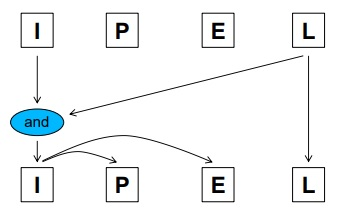
\includegraphics[width=0.4\textwidth]{img/OB-1_0.jpg}
		
		\item systém kontroluje, zda je odpovídající právo obsaženo v množině E
	\end{itemize}
	\item RBAC:
	\begin{itemize}
		\item Role Based Access Control
		\item uživatelé mají přiřazené role
		\item role mají vlastnosti jako uživatelé, ale nelze se přihlásit přímo, pouze přes "su" --- např role root
		\item uživatel se pro použití práv role musí přihlásit (musí tedy mít roli přiřazenou, a zároveň znát její heslo)
		\item role mají přiřazené profily
		\item profily mají přiřazené množiny příkazů, spustitelné pod určitými identitami a se specifickými právy
	\end{itemize}
	\item PAM
	\begin{itemize}
		\item Pluggable Authentication Modules
		\item moduly pro autentizaci, které se dají připojit ke každému programu zvlášť
		\item možnost vytvářet programy nezávisle na konkrétních autentizačních postupech
		\item konfigurace pro konkrétní program: typ modulu --- typ použití --- modul
		
		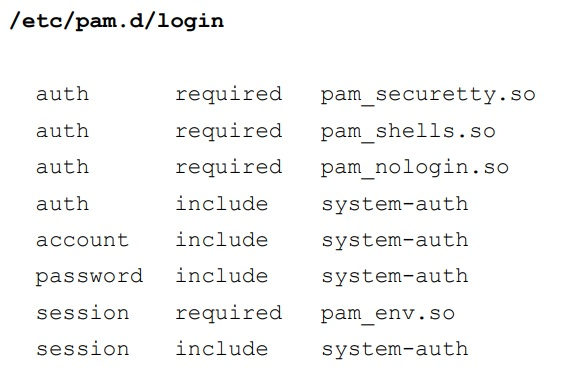
\includegraphics[width=0.6\textwidth]{img/OB-1_1.jpg}
	\end{itemize}
\end{itemize}

\newpage
\section{Šifrování a sítě}

\subsection{SP-7 (DML)}
Výroková logika: splnitelnost formulí, logická ekvivalence a důsledek, universální systém logických spojek, disjuntivní a konjunktivní normální tvary, úplné normální tvary.
\begin{itemize}
	\item \textbf{Prvotní výrok:} jednoduchá oznamovací věta, u které má smysl se ptát zda je či není pravdivá. Prvotní výroky označujeme velkými písmeny, říkáme jim \textbf{prvotní formule}.

	\item \textbf{Pravdivostní ohodnocení:} ohodnocení množiny prvotních výroků je přiřazení $v$, které každé prvotní formuli přiřadí 0 nebo 1.
	\begin{itemize}
		\item Je-li $v(A)=1$, říkáme že $A$ je pravdivý při ohodnocení $v$.
		\item Je-li $v(A)=0$, říkáme že $A$ je nepravdivý při ohodnocení $v$.
	\end{itemize}

	\item \textbf{Negace:} $\neg A$ výroku $A$ je pravdivá pro všechna ohodnocení, při kterých je $A$ nepravdivý. Pro ostatní je nepravdivá.

	\item \textbf{Konjunkce:} $A \land B$ výroků $A$ a $B$ je pravdivá pro všechna ohodnocení, při kterých jsou $A$ i $B$ současně pravdivé. Pro ostatní ohodnocení je nepravdivá.

	\item \textbf{Disjunkce:} $A \lor B$ výroků $A$ a $B$ je pravdivá pro všechna ohodnocení, při kterých je alespoň jeden z výroků $A$ a $B$ pravdivý. Pro ostatní ohodnocení je nepravdivá.

	\item \textbf{Implikace:} $A \Rightarrow B$ mezi výroky $A$ a $B$ je nepravdivá pro všechna ohodnocení, kdy \textbf{předpoklad} $A$ platí a \textbf{závěr} $B$ neplatí. Pro ostatní ohodnocení je pravdivá.

	\item \textbf{Ekvivalence:} $A \Leftrightarrow B$ mezi výroky $A$ a $B$ je pravdivá pro všechna ohodnocení, při kterých mají výroky $A$ a $B$ stejnou pravdivostní hodnotu. Pro ostatní je nepravdivá.

	\item \textbf{Tautologie ($\top$):} Formule, která je pro každé ohodnocení pravdivá.

	\item \textbf{Kontradikce ($\bot$):} Formule, která je pro každé ohodnocení nepravdivá.

	\item \textbf{Splnitelná formule:} Formule, která je alespoň pro jedno ohodnocení pravdivá.

	\item Nechť $E$ a $F$ jsou výroky. Pokud platí $E \Rightarrow F$, pak $E$ je \textbf{postačující podmínka} pro $F$. Na druhou stranu, $F$ je \textbf{nutná podmínka} pro $E$. Pokud platí $E \Leftrightarrow F$, pak je $E$ \textbf{nutná a postačující podmínka} pro $F$ a obráceně.

	\item Nechť $E$ a $F$ jsou výrokové formule. $E$ a $F$ jsou logicky ekvivalentní, právě když pro každé ohodnocení $v$ je $v(E) = v(F)$. Píšeme $E \modeleq F$.

	\item Nechť $E$ a $F$ jsou výrokové formule. $F$ je logickým důsledkem $E$, právě když pro každé ohodnocení $v$, pro které $v(E) = 1$, je i $v(F) = 1$. Píšeme $E \models F$.

	\item \textbf{Základní principy logiky:}
	\begin{itemize}
		\item Zákon vyloučení sporu: $A \land \neg A \modeleq \bot$
		\item Zákon vyloučení třetího: $A \lor \neg A \modeleq \top$
		\item Zákon dvojí negace: $\neg\neg A \Leftrightarrow A \modeleq \top$
	\end{itemize}

	\item \textbf{Obměněná implikace:} $(E \Rightarrow F) \modeleq (\neg F \Rightarrow \neg E)$

	\item Množina logických spojek tvoří \textbf{universální systém}, právě když ke každé formuli existuje logicky ekvivalentní formule, která obsahuje pouze tyto spojky.

	\item Např. dvouprvkové systémy: \{$\neg,\lor$\}, \{$\neg,\land$\}, \{$\neg,\Rightarrow$\}

	\item Existují i jednoprvkové systémy pouze z NAND ($\uparrow$) či NOR ($\downarrow$)

	\item \textbf{Literál:} Výroková formule, která je prvotní formulí, nebo negací prvotní formule.

	\item \textbf{Implikant:} Literál, či konjunkce několika literálů.

	\item \textbf{Výroková formule v disjunktivním normálním tvaru (DNT)}, pokud je implikantem, či disjunkcí několika implikantů.

	\item \textbf{Klausule:} Literál, či disjunkce několika literálů.

	\item \textbf{Výroková formule v konjunktivním normálním tvaru (KNT)}, pokud je klausulí, či konjunkcí několika klausulí.

	\item Každá výroková formule lze převést do logicky ekvivalentního KNT i DNT.

	\item \textbf{Minterm:} minterm formule $F$ je takový její implikant, který obsahuje všechny prvotní formule vyskytující se v $F$ a každou právě jednou.

	\item \textbf{Výroková formule v úplném disjunktivním normálním tvaru (ÚDNT)}, je-li mintermem nebo disjunkcí různých (logicky neekvivalentních) mintermů.

	\item \textbf{Maxterm:} minterm formule $F$ je taková její klausule, která obsahuje všechny prvotní formule vyskytující se v $F$ a každou právě jednou.

	\item \textbf{Výroková formule v úplném konjunktivním normálním tvaru (ÚDNT)}, je-li maxtermem nebo konjunkcí různých (logicky neekvivalentních) maxtermů.

	\item Každá výroková formule lze převést do logicky ekvivalentního ÚKNT i ÚDNT.
\end{itemize}
\newpage
\subsection{SP-8 (DML)}
Základy teorie čísel: dělitelnost, REA a diofantické rovnice, prvočísla, modulární aritmetika, Malá Fermatova a Eulerova věta, lineární kongruence, Čínská věta o zbytcích.

\begin{itemize}
	\item \textbf{Dělitelnost:} Nechť  $a, b \in \mathbb{Z}$. Řekneme, že $a$ dělí $b$, značíme $a \mid b$, jestliže existuje $k \in \mathbb{Z}$ takové, že $a \cdot k = b$. V takovém případě říkáme, že $a$ je (celočíselný) dělitel $b$ a b je (celočíselný) násobek $a$, případně také, že $b$ je dělitelné $a$. Pokud $a$ nedělí $b$, píšeme $a \nmid b$. Samotné $\mid$ nazýváme relací dělitelnosti.
	
	\item \textbf{Dělení se zbytkem:} Nechť $a \in \mathbb{Z}, d \in \mathbb{N}$. Pak existují jednoznačně určená čísla $q, r \in \mathbb{Z}$ taková, že $a = qd + r$ $\land$ $0 \leq r < d$. Číslo $q$ nazýváme celočíselný podíl (po dělení $a$ číslem $d$). Číslo $r \in \{0,1,...,d-1\}$ nazveme zbytkem po (celočíselném) dělení $a$ číslem $d$ a značíme jej $r = a$ mod $d$.
	
	\item \textbf{Společný dělitel:} Nechť $a, b \in \mathbb{Z}$. Číslo $n \in \mathbb{N}_0$ je společný dělitel čísel $a, b$, jestliže $n \mid a \land n \mid b$.
	
	\item \textbf{Největší společný dělitel:} Nechť $a, b \in \mathbb{Z}$. Číslo $n \in \mathbb{N}_0$ je největší společný dělitel čísel $a, b$ (značíme $n =$ gcd($a, b$)), pokud je jejich společný dělitel a současně je (celočíselným) násobkem každého jejich dalšího společného dělitele, tedy pokud $(n \mid a \land n \mid b \land (\forall d \in \mathbb{N}_0)((d \mid a \land d \mid b) \Rightarrow d \mid n))$.
	
	\item \textbf{Soudělnost:} Nechť $a, b \in \mathbb{Z}$. Nazveme je nesoudělná, pokud gcd($a, b$)$ = 1$. Pokud gcd($a, b$)$ > 1$, nazveme tato čísla soudělná.
	
	\item \textbf{Společný násobek:} Nechť $a, b \in \mathbb{Z}$. Číslo $n \in \mathbb{N}_0$ je společný násobek čísel $a, b$, jestliže $a \mid n \land b \mid n$.
	
	\item \textbf{Nejmenší společný násobek:} Nechť $a, b \in \mathbb{Z}$. Číslo $n \in \mathbb{N}_0$ je nejmenší společný násobek čísel $a, b$ (značíme $n =$ lcm($a, b$)), pokud je jejich společný násobek a současně dělí každý další jejich společný násobek, tedy pokud $(a \mid n \land b \mid n \land (\forall m \in \mathbb{N}_0)((a \mid m \land b \mid m) \Rightarrow n \mid m))$.
	
	\item \textbf{REA --- Rozšířený Euklidův Algoritmus}
	
	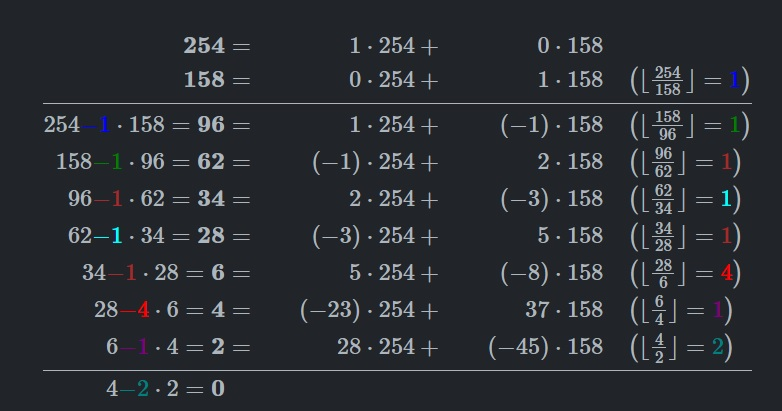
\includegraphics[width=0.6\textwidth]{img/SP-8_0.jpg}
	
	\item \textbf{LDR --- Lineární diofantická rovnice:} libovolná rovnice typu $ax+by=c$, kde $a,b,c \in \mathbb{Z}$ pro 2 neznámé $x, y \in \mathbb{Z}$.
	\begin{itemize}
		\item LDR $ax+by = c$ má alespoň jedno řešení právě tehdy když gcd($a,b$)$\mid c$.
	\end{itemize}
	
	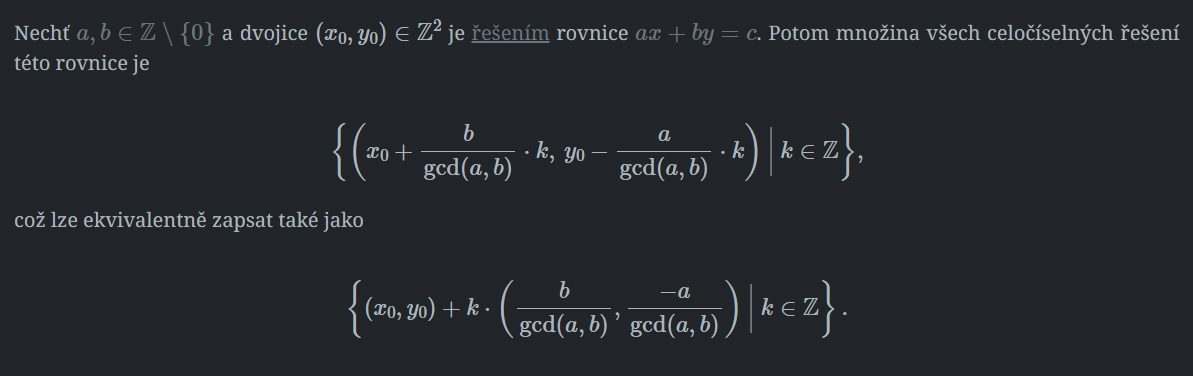
\includegraphics[width=0.9\textwidth]{img/SP-8_1.jpg}
	
	\item Přirozená čísla $\mathbb{N}$ dělíme podle počtu dělitelů do následujících 3 kategorií:
	\begin{itemize}
		\item číslo 1 (1 dělitel --- 1)
		\item \textbf{prvočísla} --- 2 dělitelé, samo číslo a 1
		\item \textbf{složená čísla} --- 3 a více dělitelů
	\end{itemize}
	\newpage
	\item \textbf{Kongruence modulo $m$:} Nechť $a,b \in \mathbb{Z}, m \in \mathbb{N}$. Pokud $m \mid (a - b)$, říkáme že $a$ je kongruentní s $b$ modulo $m$ a píšeme $a \equiv b$ (mod $m$). V opačném případě $a$ není kongruentní s  $b$ modulo $m$ a píšeme $a \not\equiv b$ (mod $m$).
	
	\item \textbf{Množina zbytků:} Nechť $m \geq 2$. Jako $\mathbb{Z}_m$ označíme množinu všech zbytků modulo $m$, $\mathbb{Z}_m = \{0,1,2,...$, $m-1\}$. Operace sčítání: součet a modulo. Násobení totéž.
	
	\item \textbf{Inverze v $\mathbb{Z}_m$:} Aditivní inverze (opačný prvek) --- součet modulo je 0. Multiplikativní inverze (inverzní prvek) --- násobek modulo je 1.
	
	\item \textbf{Existence multiplikativní inverze:} Nechť $m \geq 2$ a $a \in \mathbb{Z}_m$. V $\mathbb{Z}_m$ existuje multiplikativní inverze k $a$ právě tehdy, když gcd($a, m$) = 1. Pokud existuje, je jediná. 
	
	\item \textbf{Krácení v modulu:} Nechť $a, b, c \in \mathbb{Z}$ a $m \in \mathbb{N}, m \geq 2$, označme $d =$ gcd($m, c$). Pak platí ekvivalence: $ac \equiv bc$ (mod $m$) $\Leftrightarrow$ $a \equiv b$ (mod $m \over d$)
	
	\item \textbf{Malá Fermatova věta:} Buď $p$ prvočíslo a $a \in \mathbb{N}$ takové přirozené číslo, které není násobkem $p$ (tedy gcd($a, p$) = 1). Potom platí kongruence $a^{p-1} \equiv 1$ (mod $p$).
	
	\item Pokud je $p$ prvočíslo a $a \in \mathbb{Z}_p \land a \neq 0$, pak $a^{p-2}$ je multiplikativní inverzí čísla $a$ mod $p$. 
	
	\item \textbf{Eulerova funkce:} $\varphi$ : $\mathbb{N} \rightarrow \mathbb{N}$ je zobrazení, které každému $n \in \mathbb{N}$ přiřafí počet přirozených čísel menších nebo rovných $n$, která jsou s $n$ nesoudělná. Tedy $(\forall n \in \mathbb{N}(\varphi (n) := |\{k \in \mathbb{N} \mid k \leq n \land$ gcd($k, n$) $ = 1\}|)$.
	
	\item \textbf{Eulerova věta:} Nechť $m \in \mathbb{N}, m \geq 2$ a $a \in \mathbb{N}$ je číslo nesoudělné s $m$. potom platí kongruence $a^{\varphi(m)} \equiv 1$ (mod $m$).
	
	\begin{itemize}
		\item $p$ je prvočíslo, tedy $\varphi(p) = p - 1$
		\item $p$ je prvočíslo, $\alpha \in \mathbb{N}$, pak $\varphi(p^\alpha) = p^\alpha - p^{\alpha - 1}$
		\item $m, n \in \mathbb{N}$, gcd($m, n$) = 1. Potom $\varphi(m\cdot n) = \varphi(m) \cdot \varphi (n)$.
	\end{itemize}
	
	\item Nechť $m \in \mathbb{N}, m \geq 2$ a $a \in \mathbb{Z_m}$ je číslo nesoudělné s $m$. potom $a^{\varphi(m) - 1}$ je multiplikativní inverzí čísla $a$ mod $m$.
	
	\item \textbf{Lineární kongruence:} řešením lineární kongruence rozumíme nalezení všech celých čísel $x$ splňujících kongruenci $ax \equiv b$ (mod $m$), kde $a, b, m \in \mathbb{Z}$ a $m \geq 2$.
	
	\item \textbf{ČVOZ --- Čínská věta o zbytcích}
	
	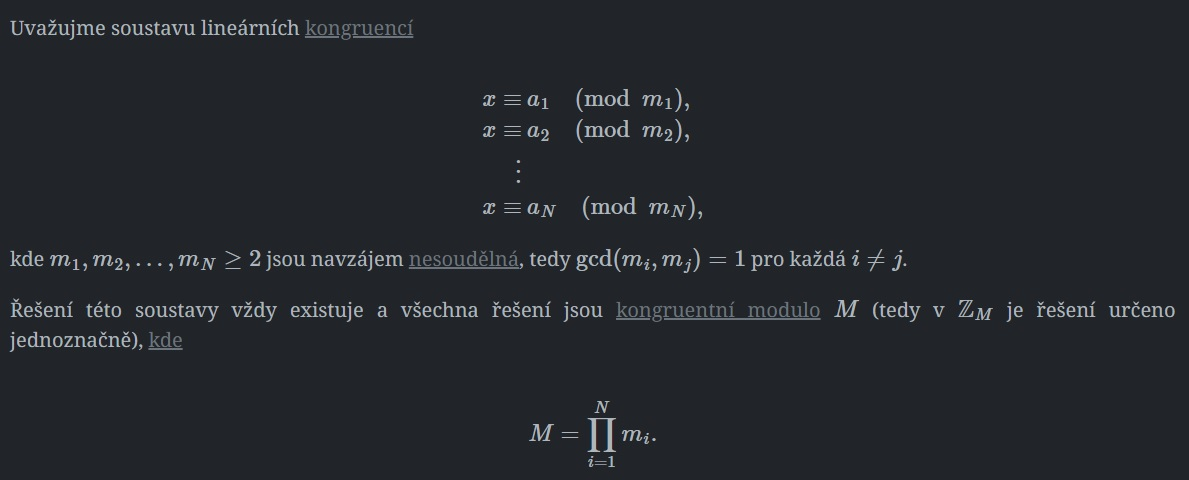
\includegraphics[width=0.9\textwidth]{img/SP-8_2.jpg}
	
	\item Výsledek je: $x = a_1 \cdot M_1 \cdot X_1 + ... + a_N \cdot M_N \cdot X_N$ (mod $M$)
	
	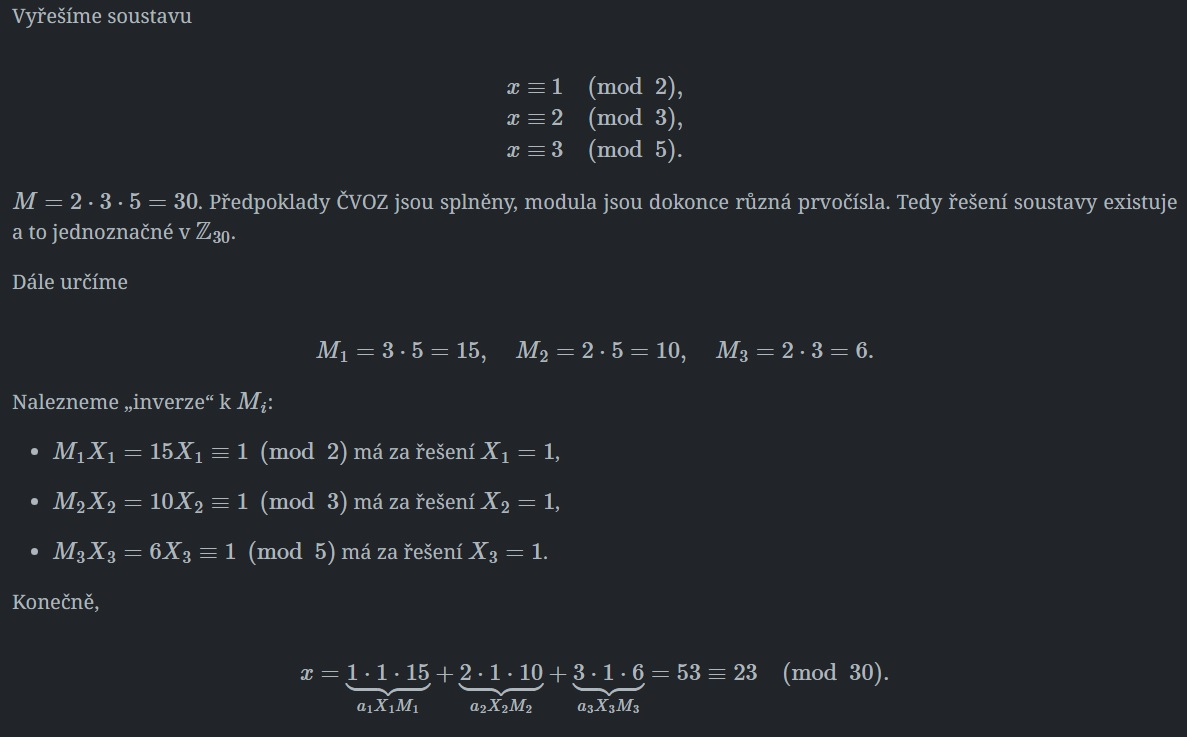
\includegraphics[width=0.9\textwidth]{img/SP-8_3.jpg}
	
	\item \textbf{ZČVOZ --- Zobecněná čínská věta o zbytcích}
	
	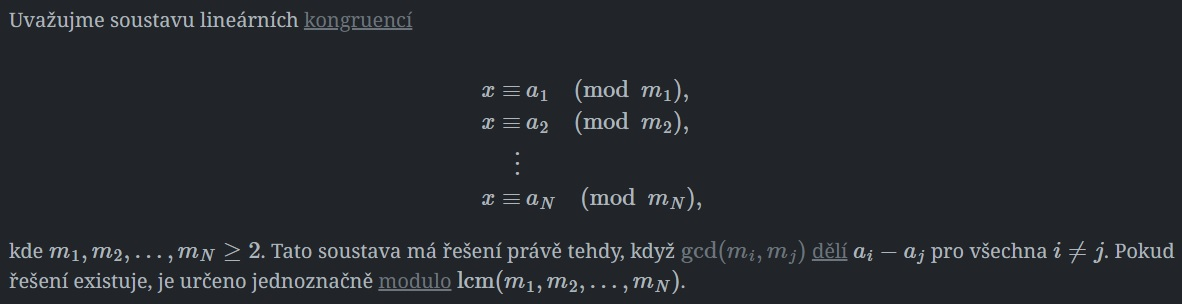
\includegraphics[width=0.9\textwidth]{img/SP-8_4.jpg}
\end{itemize}
\newpage
\subsection{SP-9 (KAB)}
Asymetrické kryptosystémy (šifra RSA, Diffie-Hellman, RSA digitální podpis), hešovací funkce (SHA-2, HMAC). Digitální podpis. Certifikáty, certifikační autority.

\subsubsection*{Asymetrické šifry}
\begin{itemize}
	\item pro šifrování a dešifrování se používají různé klíče
	\item pomocí veřejného klíče šifrujeme, promocí privátního klíče dešifrujeme
	\item privátní klíč nelze odvodit z veřejného klíče v rozumném čase
	\item každý subjekt má svůj vlastní pár veřejný-privátní klíč
\end{itemize}
\textbf{princip RSA}
\begin{itemize}
	\item šifrovací systém založený na modulárním umocňování
	\item dvojice ($e, n$) je veřejný klíč ($e$ --- veřejný exponent, $n$ --- modul)
	\item $n$ je součinem dvou velkých prvočísel $p$ a $q$, tedy $n = pq$ a gcd($e, \varphi(n)$) = 1
	\item zašifrováni plaintextu --- písmena se převedou na numerické ekvivalenty, vytvoří se bloky s největší možnou velikostí --- $E(m) = c = |m^e|_n$, $0 < c < n$ ($m$ je vytvořený blok plaintextu, $c$ je výsledný blok ciphertextu)
	\item k dešifrování je nutná znalost inverze $d$ čísla $e$ modulo $\varphi(n)$ --- gcd($e, \varphi(n)$) = 1, inverze tedy existuje --- $D(c) = |c^d|_n = |m^{ed}|_n$, $e$ a $d$ jsou inverzní modulo $\varphi(n)$, tedy $ed \equiv 1$ (mod $\varphi(n)$), tedy $ed = 1 + k \cdot \varphi(n)$, z toho $\Rightarrow |m^{ed}|_n = |m^{1 + k \cdot \varphi(n)}|_n = |m \cdot (m^{\varphi(n)})^{k}|_n$, a dle Eulerovy věty $m^{\varphi(n)} \equiv 1$ (mod $n$), tedy celkově $D(c) = |m|_n$
	
	\item dvojice ($d, n$) tvoří soukromý klíč 
	
	\item existuje možnost, že $m$ a $n$ jsou soudělné, ale je extrémně malá
\end{itemize}

\textbf{Generování RSA klíčů}
\begin{itemize}
	\item jak hledat $p$ a $q$?
	\item subjekt nalezne 2 velká náhodná čísla $p$ a $q$ s 340 dekadickými číslicemi
	\item z věty o prvočíslech plyne, že pravděpodobnost toho, že takto vybraná čísla jsou prvočísla, je cca $2 /$ log($10^340$)
	\item pro nalezení prvočísla je potřeba v průměru 1 / ($2 /$ log($10^340$)) $\approx$ 400 testů takových čísel
	\item exponent $e$ by následně měl být zvolen jako číslo větší než $p$ a $q$ --- $2^e$ by mělo být větší než $n$, aby šifrování i dešifrování muselo používat redukci modulo $n$ a nešlo pouze odmocnit
\end{itemize}

\textbf{Bezpečnost RSA}
\begin{itemize}
	\item modulární umocňování potřebné k šifrování zprávy s použitím RSA může být provedeno při velikosti modulu a bloku cca 680 dekadických číslic v řádech milisekund
	\item dešifrovací exponent $d$ nelze z dvojice ($e, n$) snadno odvodit, protože je potřeba znát hodnota $\varphi(n)$ --- pro rychlé spočítání je třeba znát faktorizaci $n = pq$
	\item i v případě cca 100-číslicových $p$ a $q$ (tedy 200-číslicového modulu $n$) trvá nejrychlejším známým algoritmům faktorizace kolem 250 let
	\item náročnost prolomení je tím větší, čím větší je modul 
	\item ochrana proti speciálním rychlým technikám faktorizace $n$: např. obě hodnoty $p-1$ a $q-1$ by měly mít velký prvočíselný faktor, tedy malé gcd($p-1, q-1$) a rozdíl $p - q$ by měl být dostatečně velký
\end{itemize}

\textbf{Digitální podpis s použitím RSA}
\begin{itemize}
	\item uvažujme 2 subjekty, každý má svůj pár privátní-veřejný klíč ($PK_1, VK_1$), ($PK_2, VK_2$)
	\item subjekt 1 chce poslat podepsanou zprávu
	\item subjekt 1 ji podepíše: $S = D_{PK_1}(m) = |m^{d_1}|_{n_1}$
	\item subjekt 1 zašifruje pro subjekt 2: $c = E_{VK_2}(S) = |S^{e_2}|_{n_2}$ (pokud $n_2 > n_1$, jinak je nutné rozdělit $S$ do bloků o velikosti menší než $n_2$ před šifrováním)
	\item subjekt 2 nejprve dešifruje svým privátním klíčem, následně použije šifrovací transformaci veřejným klíčem subjektu 1 pro odkrytí původního obsahu
	\item subjekt 2 si je tedy jistý, že zpráva přišla od subjektu 1, a zároveň subjekt 1 nemůže popřít, že danou zprávu poslal
\end{itemize}

\textbf{Urychlení RSA výpočtů}
\begin{itemize}
	\item urychlení šifrování --- doporučená množina exponentů $e$ s nízkou Hammingovou váhou
	\item urychlení dešifrování --- použití Čínské věty o zbytcích (RSA-CRT) (rozklad čísel, počítá se s čísly poloviční délky)
\end{itemize}

\textbf{Diffie-Hellmann}
\begin{itemize}
	\item algoritmus pro ustanovení společného klíče
	\item subjekt A a B si veřejně dohodnou prvočíslo $m$ a bázi $a$ ($1 < a < m$), přesněji grupu řádu $m-1$
	\item subjekt A si náhodně zvolí číslo $k_A$ takové, že $0 < k_A < m$ a gcd($k_A, m - 1$) = 1, spočítá $y_a = |a^{k_A}|_m$ a odešle ho B
	\item subjekt B si náhodně zvolí $k_B$ takové, že $0 < k_n < m$ a gcd($k_B, m - 1$) = 1, spočítá $y_B = |a^{k_B}|_m$ a odešle ho A
	\item A i B spočítají sdílený klíč $K = |{y_B}^{k_A}|_m = |(a^{k_B})^{k_A}|_m = |a^{k_A \cdot k_B}|_m = |(a^{k_A})^{k_B}|_m = |{y_A}^{k_B}|_m$
	\item útočník nemůže z $|a^{k_A}|_m$ ani z $|a^{k_B}|_m$ spočítat $K = |a^{k_A \cdot k_B}|_m$ --- tzv. Diffie-Hellmanův problém, DHP
	\item není složitější než DLP (problém diskrétního logaritmu), a zdá se že ale není ani jednodušší

\end{itemize}

\textbf{El Gamal}
\begin{itemize}
	\item vzniká úpravou Diffie-Hellman
	\item A zvolí číslo $g$ a prvočíslo $m$, $1 < g < m$, a $g$ je generátor odpovídající grupy řádu $m - 1$
	\item A si náhodně zvolí soukromý klíč $k_A$ tak, že $0 < k_A < m$, spočítá $y_A = |g^{k_A}|_m$
	\item A zveřejní uspořádanou trojici ($m, q, y_A$) jako veřejný klíč, $k_A$ je soukromým klíčem
	\item B chce odeslat A zprávu $p$
	\item B si náhodně zvolí číslo $k_B$ ($0 < k_B < m$), spočítá $y_B = |g^k_B|_m$
	\item B spočítá sdílený klíč $K = |{y_A}^{k_B}|_m = |g^{k_A \cdot k_B}|_m$ 
	\item B zašifruje zprávu $p$ pomocí vztahu $c = |p \cdot K|_m$
	\item B odešle A uspořádanou dvojici ($y_B, c$)
	\item A si spočítá $K = |{y_B}^{k_A}|_m = |g^{k_A \cdot k_B}|_m$
	\item A si spočítá $|k^{-1}|_m$ (přes REA)
	\item A dešifruje zprávu: $p = |c \cdot K^{-1}|_m = |p \cdot K \cdot K^{-1}|_m = |p|_m$
\end{itemize}

\subsubsection*{Hash funkce}
\begin{itemize}
	\item základní pojmy: jednosměrnost, bezkoliznost
	\item \textbf{Jednosměrnost:} $f: X \rightarrow Y$, je snadné z jakékoliv hodnoty $x \in X$ vypočítat $y = $ f($x$), ale je výpočetně nemožné pro náhodný obraz $y \in $f($X$) najít vzor $x \in X$, aby $y = $ f($x$)
	\item \textbf{Hashovací funkce} je jednosměrná (1. typu --- neexistují zadní vrátka pro zpětný výpočet) a bezkolizní, zároveň pro různé vstupy vrací stejně dlouhý výstup (hash)
	\item \textbf{Orákulum:} libovolná stroj, který na základě vstupu odpoví nějakým výstupem, na stejný vstup odpovídá stejným výstupem
	\item \textbf{Náhodné orákulum:} na nový vstup odpovídá náhodným výběrem z množiny vstupů
	\item Hashovací funkce se má chovat jako náhodné orákulum (bezpečnostní vlastnosti)
	\item \textbf{Bezkoliznost 1. řádu:} Hash fce $h$ je odolná proti kolizím 1. řádu, jestliže je výpočetně nezvládnutelné nalezení libovolných dvou různých (byť nesmyslných) zpráv $M$ a $M'$ tak, že $h(M) = h(M')$
	\item bezkoliznost se využívá k digitálním podpisům
	\item nepodepisuje se zpráva (moc dlouhá) ale její hash
	\item bezkoliznost zaručuje, že je složité nalézt 2 dokumenty se stejným hashem --- proto lze podepisovat hash
	\item \textbf{Bezkoliznost 2. řádu:} Hash funkce $h$ je odolná proti kolizi 2. řádu, jestliže pro jakýkoliv vzor $x$ je výpočetně nezvládnutelné nalézt 2. vzor $y \neq x$ tak, že  $h(x) = h(y)$
	\item \textbf{Odolnost pro nalezení kolize 1. řádu:} pokud se hash funkce s hashem délky $n$ bude chovat jako náhodné orákulum, složitost nalezení kolize s 50 \% pravděpodobností je $\approx 2^{\frac{n}{2}}$ (narozeninový paradox)
	\item \textbf{Odolnost proti nalezení kolize 2. řádu:} pokud se hash funkce s hashem délky $n$ bude chovat jako náhodné orákulum, složitost nalezení 2. vzoru je $\approx 2^{n}$
	\item pokud pro konkrétní hash funkci lze nalézat vzory/kolize rycheji, hovoříme o prolomení hashovací funkce
	\item při hashování se typicky zpráva rozdělí na bloky, poslední blok se doplní (např. jednou 1 a pak samé 0, aby otisky zpráv co by na konci měly např. jen víc nul byly jiné)
	\item pro konkrétní bloky se využívá kompresní funkce $f$, která z předchozího kontextu $H_{i-1}$ a bloku $M_i$ vytvoří kontext $H_i$
	\item při konstrukci hash funkce dle následujícího obrázku bezkoliznost kompresní funkce zaručuje bezkoliznost celé hashovací funkce
\end{itemize}

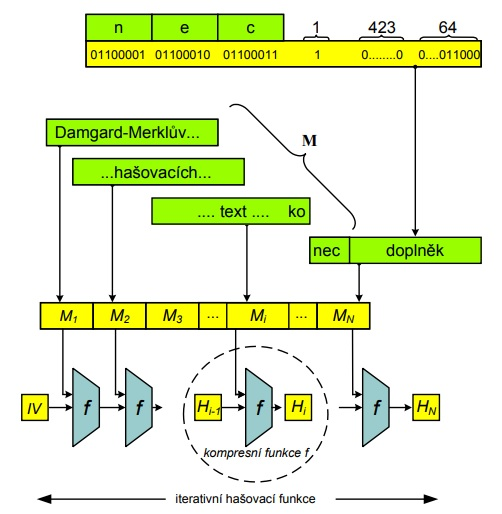
\includegraphics[width=0.55\textwidth]{img/SP-9_0.jpg}

\begin{itemize}
	\item jako kompresní funkce se typicky používá bloková šifra --- kontext $H_{i-1}$ je vstup, blok $M_i$ je klíč
	\item dle Davies-Meyerovy konstrukce se ještě po zašifrování přičte (XOR) původní kontext
\end{itemize}

\textbf{HMAC}
\begin{itemize}
	\item nepadělatelný integritní kód zprávy
	\item pro zprávu se spočítá za použití tajného klíče $K$
	\item detekuje chyby při přenosu, zabraňuje neoprávněné změně zprávy
	
	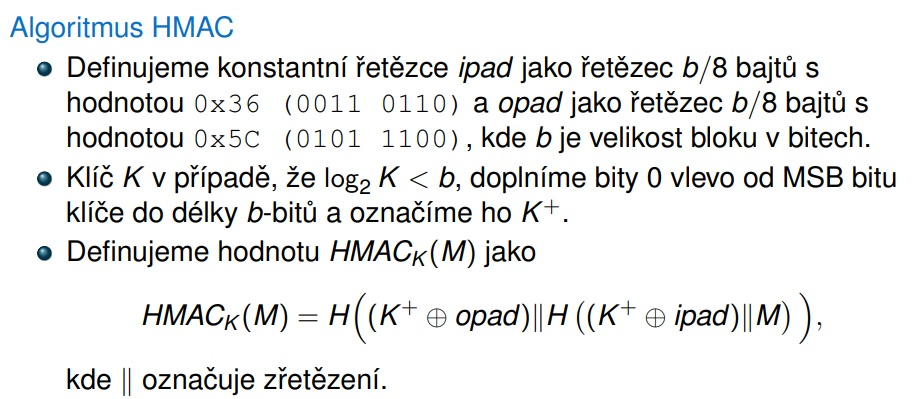
\includegraphics[width=0.7\textwidth]{img/SP-9_1.jpg}
\end{itemize}

\subsubsection*{Public Key Infrastructure}
\begin{itemize}
	\item jak distribuovat tajné symetrické klíče? distribuujeme veřejné klíče, následně si tajné klíče předáme za použití asymetrického šifrování
	\item jak distribuovat veřejné klíče? jak zabránit možnosti podvrhnutí?
	\item \textbf{Zveřejnění veřejných klíčů}
	\begin{itemize}
		\item zasílání veřejných klíčů přímo
		\item rychlé a jednoduché
		\item není odolné proti podvržení
	\end{itemize}
	\item \textbf{Veřejně dostupný adresář}
	\begin{itemize}
		\item vyšší úroveň bezpečnosti
		\item distribuci zajišťuje důvěryhodná autorita/správce
	\end{itemize}
	
	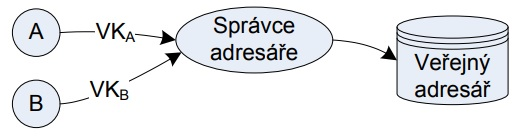
\includegraphics[width=0.4\textwidth]{img/SP-9_2.jpg}
	
	\item \textbf{Autorita pro veřejné klíče}
	\begin{itemize}
		\item přísnější dohled na distribuci veřejného klíče z adresáře
		\item autorita má svůj pár veřejný-privátní klíč, každý účastník musí znát její veřejný klíč
	\end{itemize}
	
	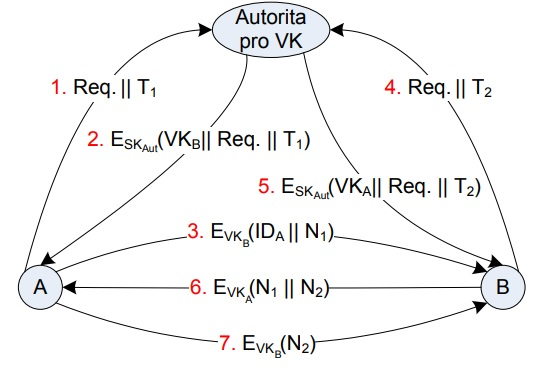
\includegraphics[width=0.45\textwidth]{img/SP-9_3.jpg}
	
	\item \textbf{Certifikace veřejných klíčů}
	\begin{itemize}
		\item distribuce veřejného klíče bez kontaktu se třetí stranou
		\item Certifikát: struktura obsahující veřejný klíč držitele, identifikační údaje držitele, dobu platnosti, další údaje vytvořené CA a zejména podpis CA
		\item Certifikační Autorita (CA): důvěryhodná třeí strana, která na základě žádosti vydává a aktualizuje certifikáty --- certifikáty vytvořené CA lze ověřit jejím veřejným klíčem	
	\end{itemize}
	
	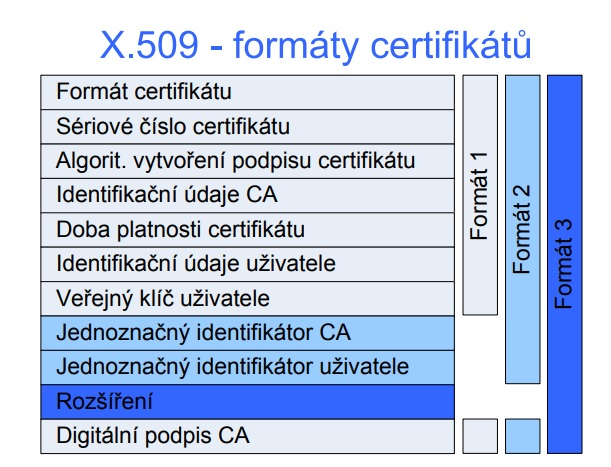
\includegraphics[width=0.5\textwidth]{img/SP-9_4.jpg}
	
	\item certifikáty mohou být podepsané ve stromové struktuře --- certifikát držitele podepsaný CA$_1$, její certifikát podepsaný CA$_2$...
	\item kořenové certifikáty musí být distribuovány jinak (typicky např. s operačním systémem)
\end{itemize}
\newpage
\subsection{SP-10 (KAB)}
Symetrické šifry blokové a proudové, základní parametry, operační módy blokových šifer, jejich základní popis a slabiny.

Symetrické šifry používají pro operaci šifrování a dešifrování stejný klíč (případně snadno převeditelný).

\subsubsection*{Proudové šifry}
\begin{itemize}
	\item proudová šifra zpracovává každý znak zvlášť
	\item na každý znak je použita jiná šifrovací transformace $E_{h_i}$, která je posunem v abecedě o $h_i$ znaků
	\item posloupnosti $h_1, h_2, ...$ se říká key-stream, a je vygenerována z klíče
	\item synchronní šifry: key-stream je závislý pouze na klíči (vypadne znak --- zbytek textu už nerozšifrujeme)
	\item asynchronní šifry: key-stream je závislý jak na klíči, tak na předchozích zpracovaných datech (takže na OT a/nebo ŠT) (vypadne znak --- po $n$ znacích jsme schopni zase dešifrovat správně)
	
	\item příklad šifer: RC4, Salsa20, ChaCha, A5/1
\end{itemize}


\subsubsection*{Blokové šifry}
\begin{itemize}
	\item šifrují $t$ znaků najednou (bloky délky $t$)
	\item všechny bloky jsou šifrovány tou samou transformací
	\item DES, 3DES --- 64b blok, DES 56b klíč, 3DES 112b/168b klíč
	\item AES --- 128b blok, 128b/192b/256b klíč
	\item šifra Feistelova typu --- postupná aplikace relativně jednoduchých operací, vytvoří poměrně složitý algoritmus
	\item iterativní bloková šifra --- základem je jednoduchá funkce provádějící šifrování jednoho bloku, která je několikrát zopakována na tom samém bloku --- jedna iterace se jmenuje 1 runda
	\item DES --- 16 rund, z 56b klíče se expandují rundovní klíče, v praxi nevýhoda krátkého klíče
	\item 3DES --- kombinace 3 operací DES za sebou, s použitím 2 nebo 3 různých DES klíčů ($E_{K_1}$, $D_{K_2}$, $E_{K_{1/3}}$)
	\item AES --- 10/12/14 rund v závislosti na délce klíče --- není Feistelova typu, nemá slabé klíče, odolná proti různým útokům
	\begin{itemize}
		\item stav = 1 blok (16B) v matici 4x4
		\item Expanze klíče --- z klíče se odvodí rundovní klíče
		\item AddRoundKey (xor rundovního klíče se stavem)
		\item Iterace/runda: SubBytes (náhrada bytů dle tabulky), ShiftRows (posunuti bytů cyklicky v řádcích), MixColumns (vynásobení matice maticí), AddRoundKey
		\item v poslední rundě je vynechána MixColumns
	\end{itemize}
	
\end{itemize}

\subsubsection*{Operační módy}
\begin{itemize}
	\item operační módy blokových šifer nám mohou zlepšit vlastnosti blokových šifer
	\item ECB (Electronic Codebook)
	\begin{itemize}
		\item bloky jsou šifrovány i dešifrovány nezávisle na sobě
		\item stejný blok OT má stejný obraz v ŠT
		\item lze zasahovat do dat --- odebírat bloky a přehazovat
		\item 1 bit chyby v ŠT poškodí celý blok OT
	\end{itemize}
	\item CBC (Cipher Block Chaining)
	\begin{itemize}
		\item je potřeba IV
		\item každý blok OT se nejprve sečte (xor) s předchozím blokem ŠT (první IV) a následně zašifruje
		\item 1 bit chyby v ŠT poškodí celý aktuální blok OT a 1 bit z následujícího
	\end{itemize}
	\item CFB (Cipher Feedback)
	\begin{itemize}
		\item je potřeba IV
		\item dělá z blokové šifry proudovou (asynchronní/samosynchronní)
		\item každý blok OT se sečte (xor) s přechozím blokem ŠT, který byl nejprve zašifrován klíčem (IV pro první blok)
		\item 1 bit chyby v ŠT poškodí celý příští blok OT a 1 bit z aktuálního
	\end{itemize}
	\item OFB (Output Feedback)
	\begin{itemize}
		\item je potřeba IV
		\item dělá z blokové šifry proudovou (synchronní)
		\item každý blok OT se sečte (xor) s aktuálním heslem z key-streamu, key-stream je nezávislý na OT i ŠT, postupně se generuje z IV operací šifrování
		\item 1 bit chyby v ŠT poškodí 1 bit v aktuálním bloku OT
	\end{itemize}
	
	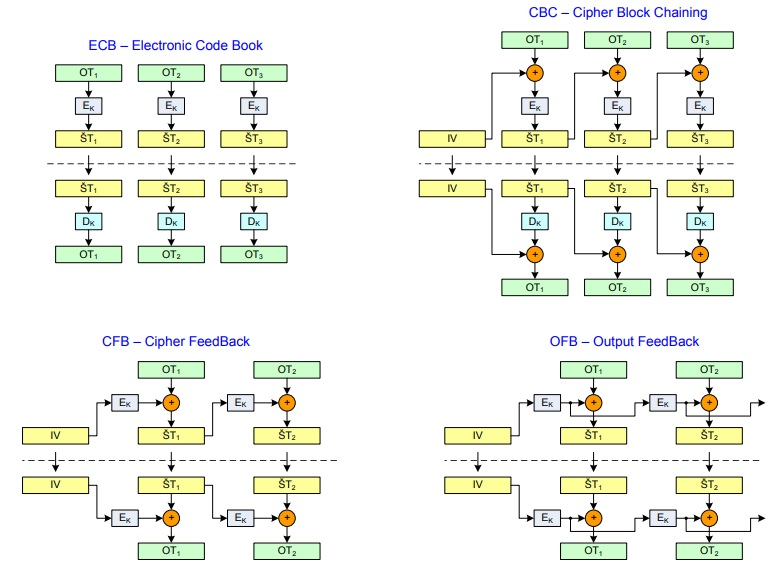
\includegraphics[width=0.9\textwidth]{img/SP-10_0.jpg}
	
	\item CTR (čítačový mód)
	\begin{itemize}
		\item dělá z blokové šifry proudovou (synchronní)
		\item každý blok OT se sečte (xor) s aktuálním heslem z key-streamu, key-stream je nezávislý na OT i ŠT, postupně se generuje použitím čítače (načte se IV, poté se něco přičítá)
		\item 1 bit chyby v ŠT poškodí 1 bit v aktuálním bloku OT
		\item má zaručit maximální periodu hesla
		\item v žádných zprávách šifrovaných tímtéž klíčem nesmí dojít k vygenerování stejného bloku hesla vícekrát --- obsah čítače nesmí být stejný
	\end{itemize}
	\item MAC (message authentication code)
	\begin{itemize}
		\item proudové i blokové šifry zajišťují důvěrnost, ne integritu zpráv
		\item MAC zajišťuje integritu a původ zprávy
		\item použije se jiný klíč než k šifrování
		\item funguje jako CBC s nulovým IV, průběžný ŠT se neodesílá
		\item MAC je tvořen posledním blokem ŠT$_n$
	\end{itemize}
	
	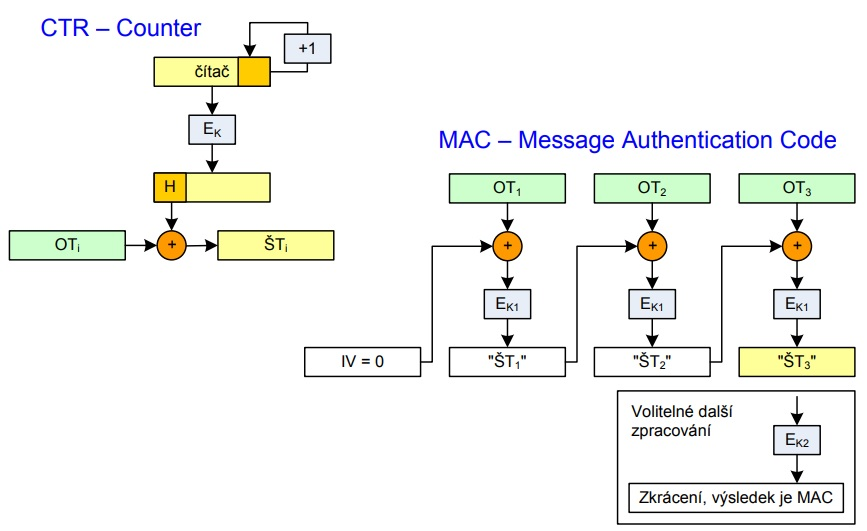
\includegraphics[width=0.9\textwidth]{img/SP-10_1.jpg}
\end{itemize}
\subsection{SP-24 (PSI)}
ISO/OSI model, enkapsulace a dekapsulace posílaných dat, princip IP adresace. Linková vrstva, podvrstvy LLC. MAC, síťová zařízení, princip přepínání. Virtuální sítě (VLAN). Síťová vrstva, směrovače, princip směrování, protokoly IPv4 a IPv6, statické a dynamické směrování.

\subsubsection*{OSI Model}
\begin{itemize}
	\item Open System Interconnection
	
	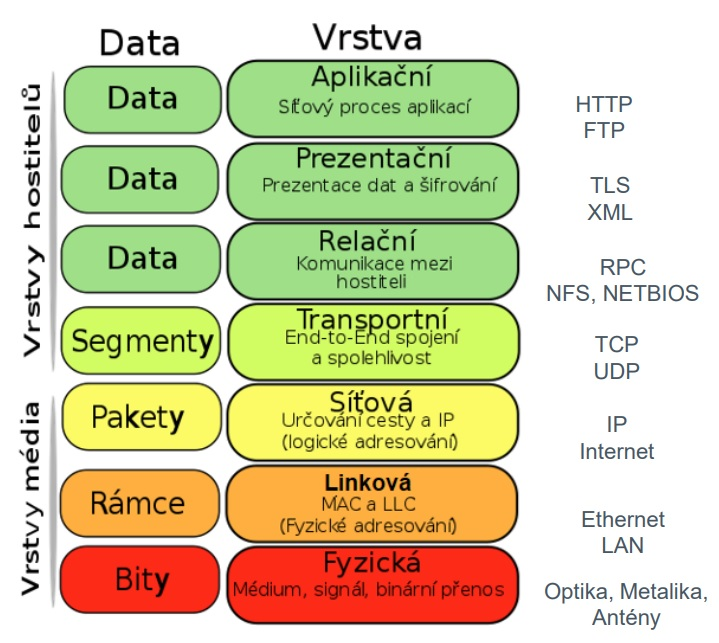
\includegraphics[width=0.6\textwidth]{img/SP-24_0.jpg}
	
	\item Aplikační vrstva --- protokoly pro komunikaci mezi aplikacemi, přenáší se data a zajímá nás význam
	\item Prezentační vrstva --- formátování a prezentace dat, šifrování, přenáší se data a zajímá nás struktura
	\item Relační vrstva --- logické rozhraní pro aplikace, RPC, sdílení filesystému, přenáší se data
	\item Transportní vrstva --- data jsou rozložena na segmenty, typicky protokol transportní vrstvy přidá nějakou hlavičku, posílá se z portu na port, řeší se E2E spojení a spolehlivost
	\item Síťová vrstva --- segmenty vyšších vrstev rozděleny na pakety, posílají se na síťovou adresu (IP)
	\item Linková vrstva --- pakety rozděleny na rámce (frames), opět přidána hlavička, posílá se na linkovou adresu (MAC)
	\item Fyzická vrstva --- převod rámců na bity a posílání přes médium (kabel, vzduch)
	
\end{itemize}

\textbf{TCP/IP model}
\begin{itemize}
	\item pouze 4 vrstvy: aplikační (první 3 OSI), transportní, internetová a síťová (spodní 2 OSI)
\end{itemize}

\subsubsection*{IP adresace}
\begin{itemize}
	\item IPv4 adresa --- 4 byty
	\item stanice v IPv4 síti se sdružují do podsítí
	\begin{itemize}
		\item adresní rozsah sítě --- skupina všech IP adres, které patří do stejné sítě
		\item maska --- určuje rozsah, je stejně dlouhá jako IP adresa, používá se prefixová notace (aaa.bbb.ccc.ddd /mm --- mm je počet bitů masky od začátku, které jsou 1)
		\item adresa sítě --- získá se z adresy nějakého zařízení v síti operací AND s maskou --- nejnižší adresa v daném rozsahu
		\item broadcast --- nejvyšší adresa z rozsahu
	\end{itemize}
\end{itemize}

\subsubsection*{Linková vrstva}
\begin{itemize}
	\item přenášení dat v rámci lokální (LAN) sítě
	\item základní přenášená jednotka je rámec (frame)
	\item skládá se z 2 podvrstev: MAC a LLC
	\item MAC:
	\begin{itemize}
		\item Medium Access Control
		\item zajišťuje přístup k médiu (fyzické vrstvě)
		\item řeší fyzickou adresaci pomocí MAC adres
		\item filtrování MAC adres
		\item plánování rámců do front  a jejich odesílání
		\item VLAN
		\item svázána s konkrétní technologií fyzické vrstvy
		\item řeší sdílený přístup k médiu (multiplex --- řešení kolizí --- časový, frekvenční, kódový, prostorový)
		\item další metody přístupu k společnému médiu --- Carrier Sense Multiple Access (CSMA (-/CD/CA))
		
		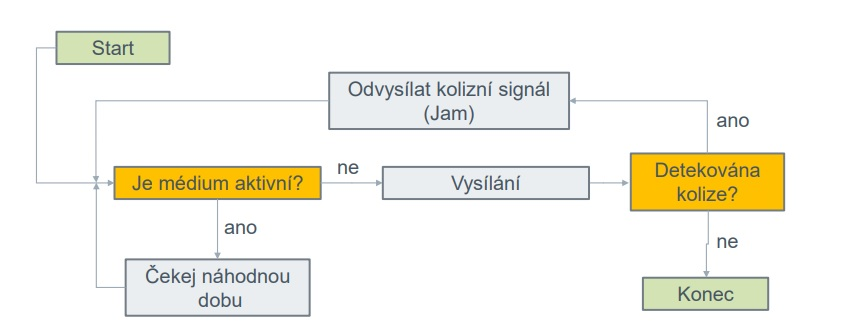
\includegraphics[width=0.6\textwidth]{img/SP-24_1.jpg}
	\end{itemize}
	\item LLC:
	\begin{itemize}
		\item Logical Link Control
		\item umožňuje existenci různých protokolů nad společnou MAC vrstvou
		\item řízení toku a kontrola chyb
		\item rozdělení toku dat z vyšších vrstev do rámců, určení velikosti rámce a jeho zakončení
		\item zajištění doručení dat --- potvrzovací schémata
		\begin{itemize}
			\item jednotlivé potvrzování (stop \& wait)
			\item selective repeat
			\item Go-Back-N
			\item klouzavé okénko
		\end{itemize}
	\end{itemize}
	\item Zařízení na linkové vrstvě:
	\begin{itemize}
		\item pracují s rámci
		\item obecný formát: hlavička, data, konec rámce (obsahuje např kontrolní součet)
		\item switch --- porty, které mají buffery --- přepínací tabulka, aby věděl kam posílat dál, switch se učí --- různé režimy přeposílání (store and forward, cut through, fragment free)
		\item bridge
	\end{itemize}
	\item broadcastová doména --- množina stanic dané sitě, kterým je doručen rámec s broadcastovou adresou
	\item v síti nesmí být smyčky, lze odstranit přes SPT (spanning tree protocol), udělá kostru
	\item MAC adresa: 6 bytů, první 3 identifikují výrobce
	
	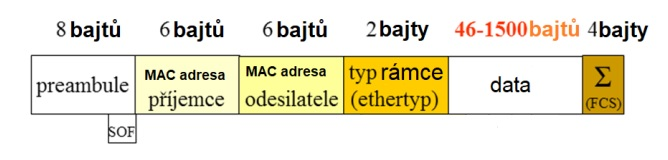
\includegraphics[width=0.6\textwidth]{img/SP-24_2.jpg}
\end{itemize}

\subsubsection*{VLAN}
\begin{itemize}
	\item každý port na switchi se dá zařadit do VLAN
	\item trunk port podporuje více (všechny) VLAN
	\item trunkem chodí označené rámce (tagged), k workstations chodí neoznačené
	\item pro přeposílání dat mezi VLAN se musí chodit přes router
	\item VLAN může být dána jak portem, tagem, tak MAC adresou nebo protokolem vyšší úrovně
\end{itemize}

\subsubsection*{Síťová vrstva}
\begin{itemize}
	\item doručuje data jak v lokální síti, tak mezi sítěmi
	\item schémata IP adresace: prefixová a dle třídy

	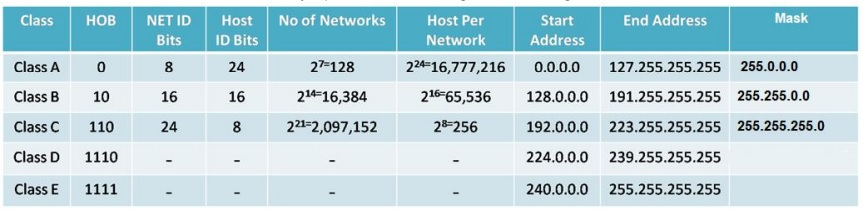
\includegraphics[width=0.8\textwidth]{img/SP-24_3.jpg}	
	
	\item speciální rozsahy:
	\begin{itemize}
		\item privátní (10.0.0.0/8, 172.16.0.0/12, 192.168.0.0/16)
		\item link-local (169.254.0.0/16)
		\item loop-back (127.0.0.0/8)
		\item multicast (224.0.0.0/4)
	\end{itemize}
	
	\item hlavička IP paketu:
	
	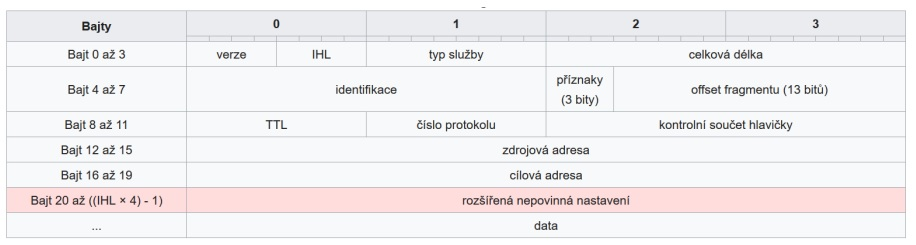
\includegraphics[width=0.8\textwidth]{img/SP-24_4.jpg}
	
	\item princip směrováni:
	\begin{itemize}
		\item směrování (routing) --odeslání konkrétního paketu prostřednictvím zvoleného síťového rozhraní na základě cílové IP adresy paketu
		\item provádí router
		\item podle toho, zda cílová adresa patří do sítě routeru se paket buď pošle cílové stanici, nebo dalšímu routeru podle směrovací tabulky
		\item směrovací tabulka má záznamy o sítích, a jakým způsobem se k nim dostat (kam a jak poslat paket)
		\item ruční zadání informací do tabulky = statické směrování
	\end{itemize}
	\item NAT (Network Address Translation) --- překlad adres na routeru z veřejné (adresa routeru) na privátní (za routerem, adresy v soukromé síti)
	\item ICMP (Internet Control Message Protocol) --- utility ping a tracert/traceroute
	\item ARP (Address Resolution protocol) --- chceme poslat paket na IP adresu, ale neznáme MAC adresu, tak se zeptáme přes MAC broadcast "kdo má tuto IP" ... cíl odpoví už ne přes broadcast že on má tuto adresu, tedy uložíme do ARP table
	\item DHCP (Dynamic Host Control Protocol) --- dynamické nastavení IP adresy a nastavení sítě pro stanici (4 zprávy, vše broadcast)
\end{itemize}

\subsubsection*{Směrování}
\begin{itemize}
	\item typy směrování:
	\begin{itemize}
		\item Redundantní --- existuje více cest do cíle
		\item symetrické --- cesta tam je stejná jako zpět
		\item asymetrické --- cesty tam a zpět se liší
		\item proaktivní --- používá směrovací tabulky, předpočítá/ví cestu do cíle (běžně v počítačových sítích)
		\item reaktivní --- zjišťuje cestu až na základě žádosti (např. v mobilních sítích)
	\end{itemize}
	\item Dynamické směrování --- algoritmy:
	\begin{itemize}
		\item Distance Vector algoritmy (např. RIP --- routing information protocol) --- routery si vymění navzájem info o vzdálenosti všech sousedů, dělají to i za běhu, tedy + router i - router, vzdálenost je pouze počet routerů v cestě
		\item Link-State algoritmy (např. OSPF) --- sestaví graf sítě i s ohodnocením hran (linkstate udaná správcem sítě)
		\item Path Vector algoritmy (např. BGP) --- routery si vyměňují celé cesty ke konkrétním cílům
	\end{itemize}
\end{itemize}

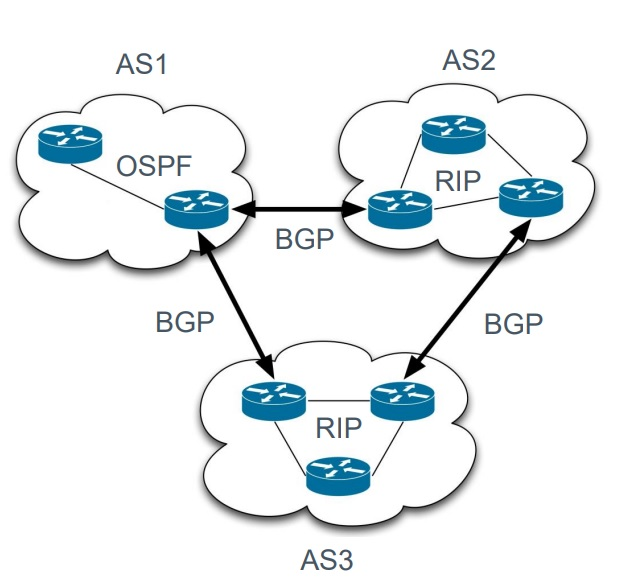
\includegraphics[width=0.6\textwidth]{img/SP-24_5.jpg}

\subsubsection*{IPv6}
\begin{itemize}
	\item umožňuje zřetězit hlavičky, hlavička je jednodušší
	\item 128b adresy (16B)
	\item není potřeba NAT
	\item umožňuje objevování sousedů, efektvnější seměrování, ...
\end{itemize}
\subsection{SP-25 (PSI)}
Transportni vrstva, protokol TCP, spolehlivost doručení paketů, zahlcení, srovnání s protokolem UDP. Překlad síťových adres (NAT) na síťové a transportní vrstvě. Systém doménových jmen (DNS).

\subsubsection*{Transportní vrstva}
\begin{itemize}
	\item zajišťuje doručení dat konkrétním aplikacím (přidává k IP adrese ještě port)
	\item řeší spolehlivost dodání dat
	\begin{itemize}
		\item možnost stop and wait --- jednoduchá, ale neefektivní, doručuje data přesně v pořadí jak jdou za sebou
		\item možnost stop and go --- nezajistí, že data dorazí do cíle, přijímač posílá vysílači stop a go signály
		\item sliding window --- okénko o nějaké velikosti, první se odesílá, na poslední se čeká na ACK
	\end{itemize}
\end{itemize}

\subsubsection*{TCP}
\begin{itemize}
	\item nejznámější protokol transportní vrstvy, který zajišťuje spolehlivé doručení dat
	\item garantuje jak doručení, tak pořadí paketů
	\item je duplexní, obě strany jsou vysílačem i přijímačem
	\item navazování a ukončování spojení:	
	
	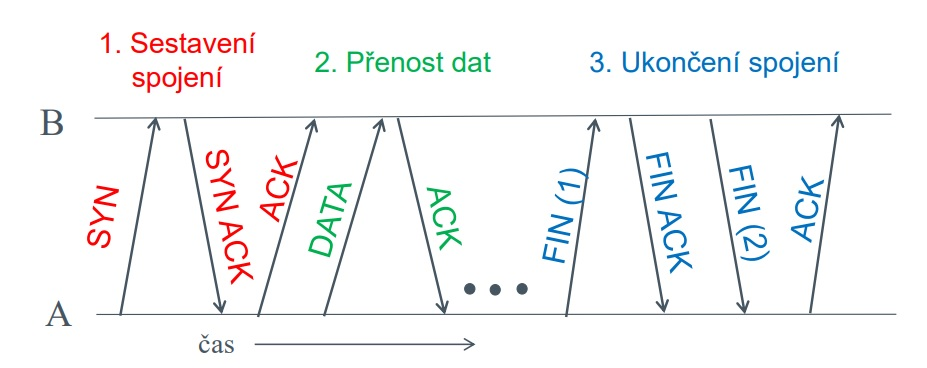
\includegraphics[width=0.8\textwidth]{img/SP-25_0.jpg}
	
	\item struktura TCP paketu
	
	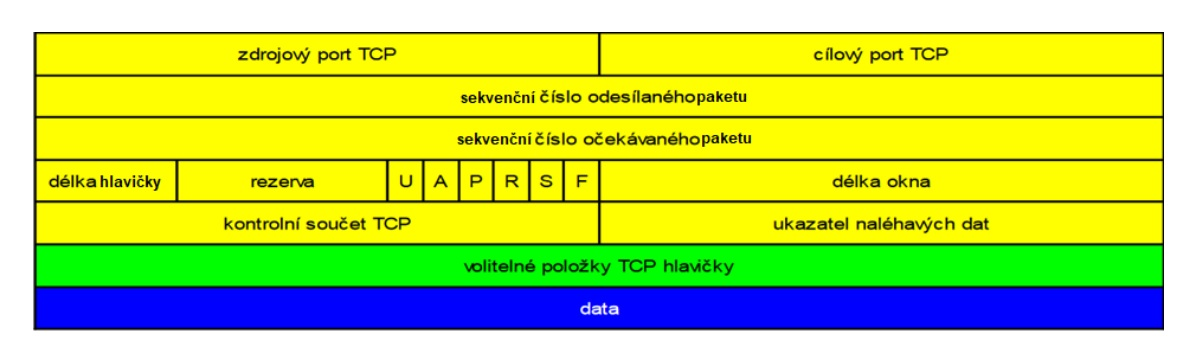
\includegraphics[width=0.8\textwidth]{img/SP-25_1.jpg}
	
	\item pro řízení toku se používá mechanismus klouzavého okénka (sliding window) --- přijímač nastavuje délku okénka dle svých možností
	
	\item vysílač ještě musí nějak zajistit, aby se nepřetížila linka, to je složitější a liší se to dle varianty TCP --- nastavuje se CWL (congestion window length)
	\item některé druhy obnovují rychlost (velikost CWL) po výpadku rychleji, jiné pomaleji
	
	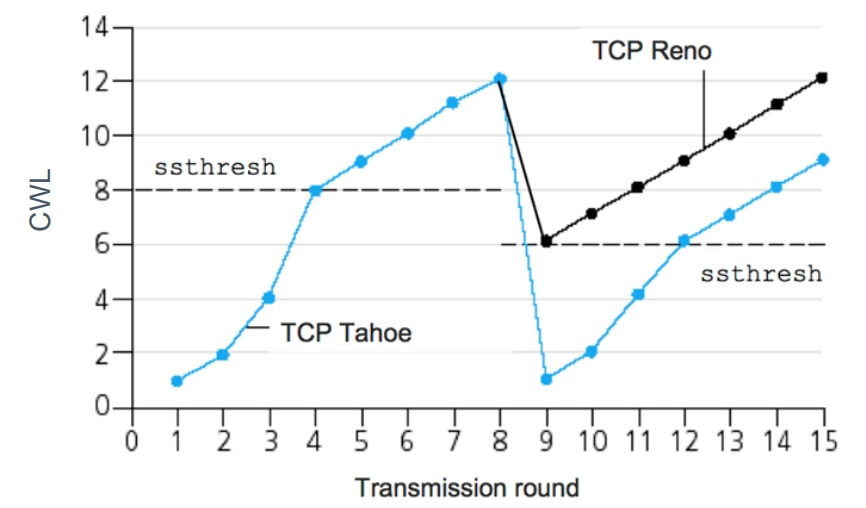
\includegraphics[width=0.6\textwidth]{img/SP-25_2.jpg}
	
\end{itemize}

\subsubsection*{UDP}
\begin{itemize}
	\item nižší režie --- vyšší propustnost než TCP
	\item běžně se používá na přenos hlasu či videa
	\item struktura UDP paketu:
	
	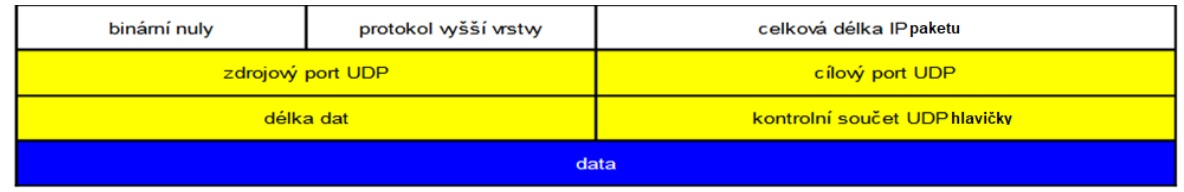
\includegraphics[width=0.8\textwidth]{img/SP-25_3.jpg}
\end{itemize}

\subsubsection*{NAT}
\begin{itemize}
	\item díky transportní vrstvě a portům je možné na routeru překládat IP adresy pro více spojení a stanic za routerem
	\item směrem ven se přeloží IP adresa, pokud je to nutné tak i port
	\item tím se vytvoří mapování na routeru --- tento výstupní port je mapován ke konkrétní IP a portu za routerem
	\item při odpovědi se dle portu rozhodne na jakou IP (a port) data poslat
\end{itemize}

\subsubsection*{DNS}
\begin{itemize}
	\item IP adresy jsou špatně zapamatovatelné
	\item DNS --- Domain Name System je primárně určen k překladu doménových jmen na IP adresy a naopak
	\item DNS je hierarchický a nezabezpečený
	\item DNS je zásadní i pro další služby jako email
	\item běží typicky na portu 53 a většina implementací využívá UDP
	
	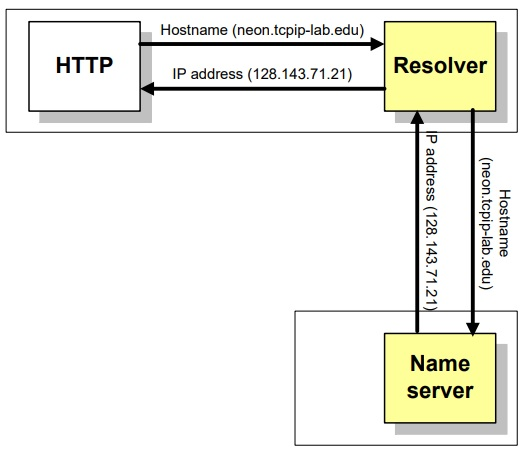
\includegraphics[width=0.5\textwidth]{img/SP-25_4.jpg}
	
	\item hierarchie domén:
	
	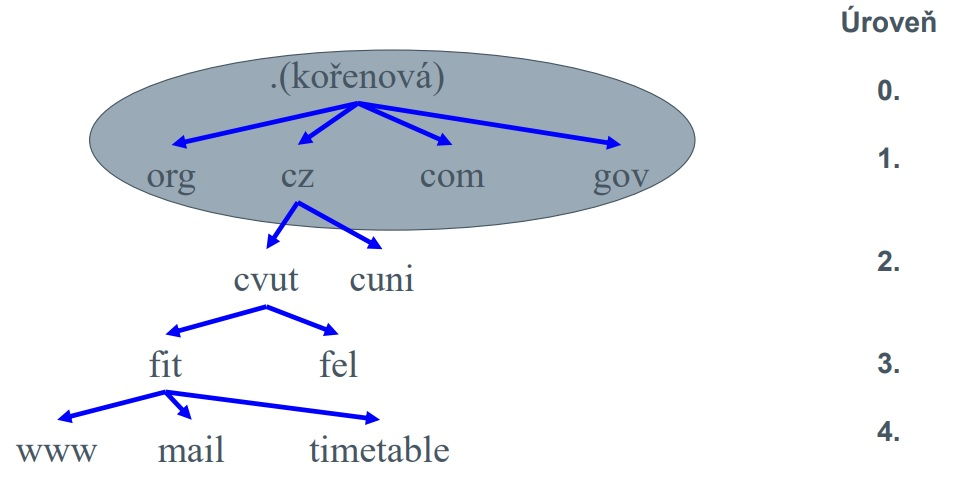
\includegraphics[width=0.7\textwidth]{img/SP-25_5.jpg}
	
	\item 4 typy Top Level Domains (TLD) (1. úrovně)
	\begin{itemize}
		\item Generic TLD (gTLD) --- 3 znaky označující funkci organizace (gov, mil, edu, org, com, net)
		\item Country Code TLD --- 2 znaky označující zemi (cz, us, de, eu)
		\item New Generic TLD --- libovolný řetězec (max 63 znaků)
		\item reverzní doména --- in-addr.arpa
	\end{itemize}
	\item dříve centralizovaný systém všech domén v souboru hosts.txt
	\item existuje iterativní způsob dotazování (dotaz lokálnímu DNS serveru, ten se postupně od root zeptá všech nutných dalších DNS serverů) nebo rekurzivní (zeptají se v řadě za sebou, lokální rootu, root TLD atd atd)
	\item existuje DNSSEC --- zabezpečený DNS (přes asymetrickou kryptografii)
	\item existuje dynamické DNS (DynDNS) --- pro případ zařízení, která často mění IP adresu
\end{itemize}
\subsection{OB-11 (ASB)}
LAN z hlediska kybernetické bezpečnosti. Zranitelnosti protokolů rodiny TCP/IP. Zabezpečení sítí LAN na úrovni síťových zařízení (switche, routery, firewally). Využití technologie VLAN.

\subsubsection*{model CIA}
\begin{itemize}
	\item Confidentiality (Důvěrnost)
	\begin{itemize}
		\item porušení důvěrnosti: odposlech síťového provozu
		\item různá úroveň informací v závislosti na vrstvě: aplikační (čtení uživatelských dat), transportní (informace o protistranách a službě), síťová (protistrany, typ transportního protokolu, velikost), ...
		\item nemusí jít vždy jen o uživatelská data, ale např informace směrovacích protokolů
	\end{itemize}
	\item Integrity (Integrita)
	\begin{itemize}
		\item data jsou nezměněna v průběhu přenosu
		\item porušení integrity: úprava přenášených dat
	\end{itemize}
	\item Availability (Dostupnost)
	\begin{itemize}
		\item běžící služba, přenos dat sítí (prostě to funguje)
		\item porušení dostupnosti: DoS (Denial of Service)
	\end{itemize}
\end{itemize}

\subsubsection*{Bezpečnost síťových protokolů}
\begin{itemize}
	\item Ethernet
	
	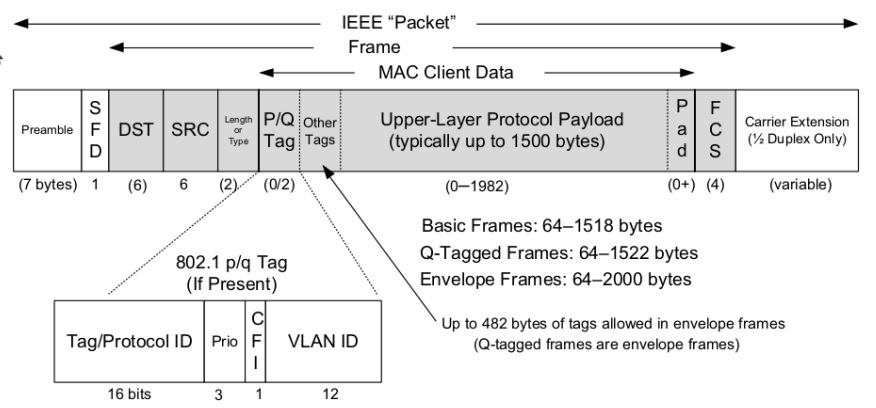
\includegraphics[width=0.8\textwidth]{img/OB-11_0.jpg}
	
	\begin{itemize}
		\item otevřená (plaintext) komunikace
		\item zajišťuje doručení dat (kontrolní součty), ale data lze jak odposlouchávat tak měnit
		\item u protokolu CSMA/CD lze udělat DoS (místo náhodné doby čekání prostě vysílat hned)
		\item lze použít VLAN --- k packetům se přidají tagy (do jaké VLAN packet patří) --- max 4094 VLAN (12 bitů, 2 rezervované hodnoty) --- rozdělení broadcastové domény
	\end{itemize}
	
	\item IP
	
	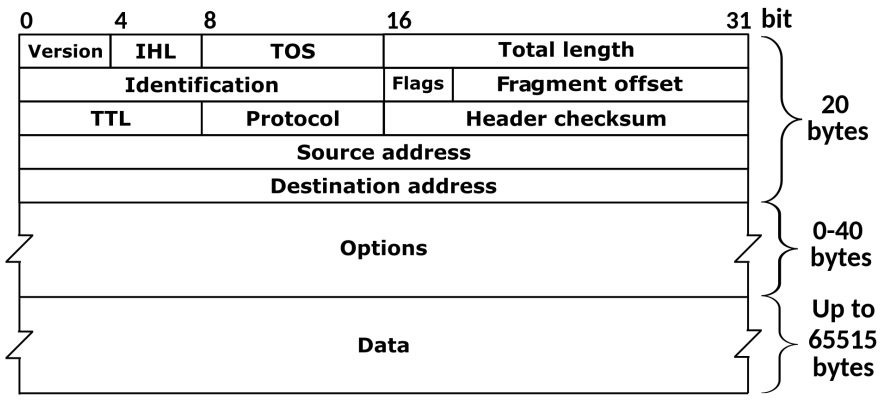
\includegraphics[width=0.7\textwidth]{img/OB-11_1.jpg}
	
	\begin{itemize}
		\item otevřená (plaintext) komunikace
		\item pouze zapouzdření a přenos dat, neřeší ani správné doručení
		\item kontrola integrity musí být zajištěna vyšší vrstvou
		\item IP adresu lze podvrhnout
	\end{itemize}
	
	\item UDP
	\begin{itemize}
		\item v hlavičce prakticky jen zdroj, cíl a checksum
		\item slouží pouze k zapouzdření dat, není garantováno pořadí
		\item integritu musí řešit vyšší vrstva
		\item nenáročný na správu spojení (lze využít k DDoS)
	\end{itemize}
	
	\item TCP
	
	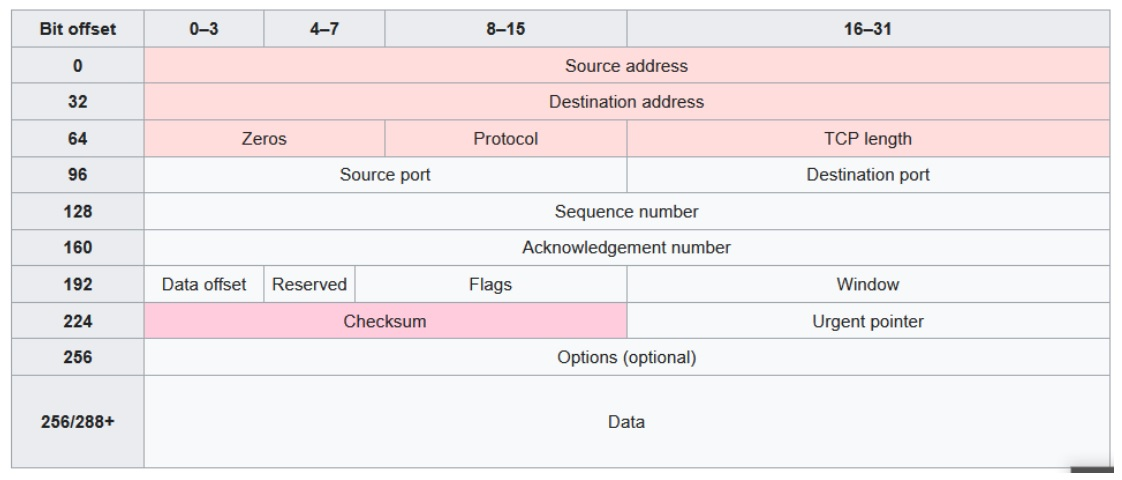
\includegraphics[width=0.7\textwidth]{img/OB-11_2.jpg}
	
	\begin{itemize}
		\item slouží pro doručení v pořadí, neřeší integritu
		\item integritu musí řešit vyšší vrstva
		\item komunikující uzly si musí uchovávat informaci o stavu spojení --- lze využít k SYN Flood DoS útoku
	\end{itemize}
	
	\item ARP
	\begin{itemize}
		\item ARP cache --- každý uzel si zapisuje příchozí odpovědi (jakékoliv)
		\item ARP Spoofing --- podvržení linkové adresy
		\item ARP Cache Poisonong --- zneužití ARP Cache oběti pomocí spoofingu --- výsledkem je zasílání dat na špatnou linkovou adresu, umožňuje získat pozici MitM (Man in the Middle)
		\item obrana: static ARP, kontrola na portu switche
	\end{itemize}
	
	\item DHCP
	\begin{itemize}
		\item DHCP server přiděluje dynamicky konfiguraci sítě zařízením
		\item rogue DHCP server --- DHCP server navíc, může vzniknout špatnou konfigurací, nebo útokem
		\item obrana: DHCP Snooping na switch portu, filtrování DHCP komunikace
	\end{itemize}
	
	\item ICMP
	\begin{itemize}
		\item nepřenáší data vyšší vrstvy, ale může přímo i nepřímo sloužit k útokům
	\end{itemize}
\end{itemize}

\subsubsection*{Bezpečnost síťových zařízení}
\begin{itemize}
	\item hub
	\begin{itemize}
	\item pracuje na fyzické vrstvě, přeposílá vstup
		\item dnes už se moc nesetkáváme, překonané zařízení
		\item bezpečnost 0, rozšiřuje kolizní doménu, každá stanice "slyší" vše co se v dané kolizní doméně děje, může způsobovat kolize úmyslně
	\end{itemize}
	\item switch
	\begin{itemize}
		\item pracuje na linkové vrstvě
		\item rámce jsou přeposílány na konkrétní port na základě paměti switche
		\item broadcast přeposílán všude
		\item odděluje kolizní domény, nedochází ke kolizím
		\item možnosti útoků typu ARP spoofing  / MAC floding
		\item široké možnosti bezpečné konfigurace switche
		\begin{itemize}
			\item vypnutí nepoužitých portů / zásuvek (aby se do volné zásuvky nemohl připojit kdokoliv)
			\item limit počtu MAC adres na portu (obrana proti MAC flooding)
			\item VLAN --- logické členění síťových segmentů, rozdělení broadcastových domén (útok VLAN hopping --- switch spoofing, pc se tváří jako switch a chce nastavit trunk spojení / double tagging, přidání extra vlan tagu)
			\item spanning tree protocol --- potřeba nastavit, aby se nemohl připojit nový (útočníkův) switch
			\item lze nastavit ochranu proti DHCP spoofingu
		\end{itemize}
	\end{itemize}
	\item router
	\begin{itemize}
		\item možnost nastavení ACL
	\end{itemize}
	\item firewall
	\begin{itemize}
		\item možnost nastavení ACL
	\end{itemize}
	\item IDS (Intrusion detection system)
	\item IPS (Intrusion prevention system)
\end{itemize}
\subsection{OB-12 (ASB)}
Kryptografické síťové protokoly, využití šifrování a algoritmu Diffie-Hellman. Protokoly TLS a SSH.

\subsubsection*{Šifrování na různých vrstvách}
\begin{itemize}
	\item šifrování na vrstvě $x$ znamená ukrytí dat vrstvy $x+1$
	\item aplikační vrstva --- šifrování řeší aplikace sama, šifrování jsou různá, závislá na aplikaci
	\item transportní vrstva --- SSL/TLS, ukrývá data a protokol aplikace
	\item síťová vrstva --- některé VPN, IPsec --- ukrývá data transportní vrstvy
	\item linková vrstva --- Wi-Fi
\end{itemize}

\subsubsection*{TLS}
\begin{itemize}
	\item šifrování na transportní vrstvě
	\item TLS se skládá z následujících vrstev:
	
	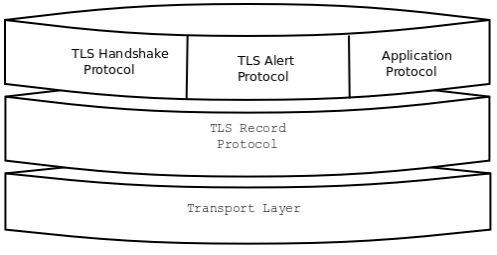
\includegraphics[width=0.6\textwidth]{img/OB-12_0.jpg}
	
	\item Record Layer --- vrstva zodpovědná za posílání TLS zpráv, skládá se z z dalších vrstev
	\item Handshake Protocol --- výběr šifrovací sady, parametrů spojení a ustanovení společných klíčů
	\item Alert Protocol --- přenos chybových zpráv, např. neplatný certifikát
	\item Application Protocol --- šifrovaný protokol aplikační vrstvy
	\item TLS handshake:
	
	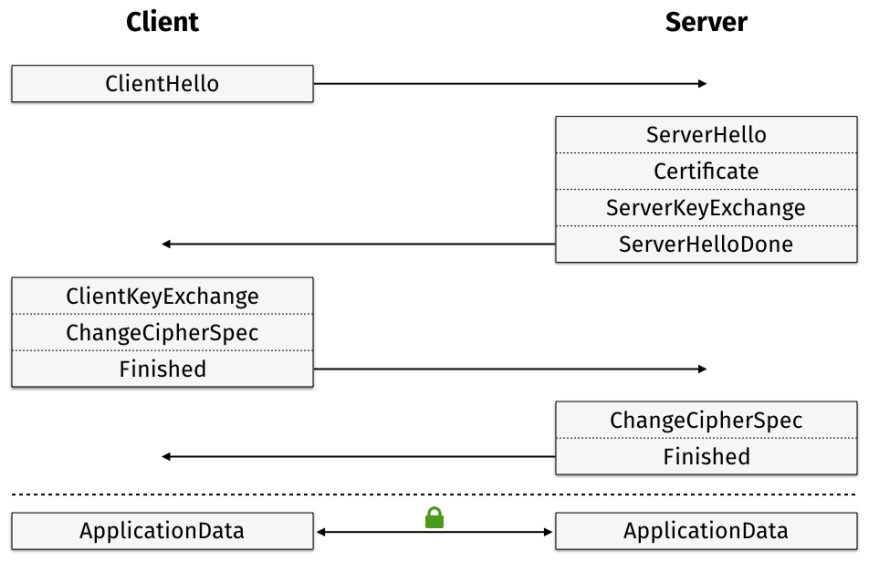
\includegraphics[width=0.8\textwidth]{img/OB-12_1.jpg}
	
	\begin{itemize}
		\item Client Hello --- obsahuje aktuální (UNIXový) čas, náhodné číslo (28B), podporované šifrovací sady a rozšíření
		\item Server Hello --- obsahuje aktuální (UNIXový) čas, náhodné číslo (28B) a podporované šifrovací sady
		\item Certifikát serveru
		\item ServerKeyExchange --- parametry serveru pro ustanovení klíčů (Diffie-Hellman)
		\begin{itemize}
			\item dle Diffie-Hellamn server stanoví hodnoty $p$ (prvočíslo) a $G$ (generátor)
			\item server vygeneruje náhodné číslo $a$ a vypočítá $Y_a = |G^a|_p$
			\item výsledné číslo podepíše svým soukromým klíčem (hash(client\_random + server\_random + server\_params)) a odešle
		\end{itemize}
		\item ServerHelloDone --- konec serverKeyExchange
		\item ClientKeyExchange --- klient spočítá svoje $Y_b = |G^b|_p$ a odešle
		\item v tuto chvíli obě strany mají společnou hodnotu $Y = |G^{a \cdot b}|_p$, která se nazývá pre-master secret
		\item z pre-master secret a z náhodných čísel se pomocí pseudo-random function vygeneruje master secret (či blok klíčů dle potřeby vybraných šifrovacích funkcí)
		\item client ChangeCipherSpec --- poslední nešifrovaná zpráva od klienta
		\item client Finished --- obsahuje hash všech předchozích zpráv + řetězec "client finished" --- slouží pro ověření funkčnosti šifrování a jako ochrana proti replay a tampering útokům
		\item server ChangeCipherSpec a Finished --- podobně jako client
		\item pro Diffie-Hellamn je možné použít vždy stejné hodnoty a a/nebo b (static-static, ephemeral-static), ale po kompromitaci kteréhokoliv private-key by šly dešifrovat i zpětně veškerou komunikaci, proto se od TLS 1.3 musí vždy generovat nové (ephemeral-ephemeral) --- (perfect) forward secrecy
	\end{itemize}
	\item TLS 1.3
	\begin{itemize}
		\item povinné použití perfect forward secrecy
		\item navíc povinné některé šifrové sady
		\item navíc AEAD šifry (Authenticated encryption with associated data)
		\item odebraly se nepoužívané funkce jako komprese
		\item odebrala se statická výměna klíčů
		\item odebral se operační mód CBC, šifry RC4, DES, 3DES, hashe MD5, SHA-1, SHA-224
		\item odebraly se slabé a nepoužívané eliptické křívky
		\item zjednodušení TLS Handshake
		
		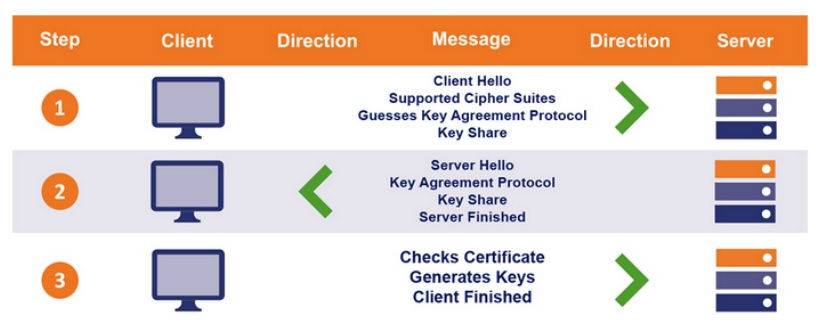
\includegraphics[width=0.8\textwidth]{img/OB-12_2.jpg}
	\end{itemize}
\end{itemize}

\subsubsection*{SSH}
\begin{itemize}
	\item Secure Shell Protocol
	\item TCP port 22
	\item transportní vrstva --- typicky běží přes TCP
	\item autentikační vrstva --- řeší autentikaci uživatele a šifrovací algoritmy, řeší autentizaci serveru
	\item spojovací vrstva --- koncept kanálů a služeb , více současných obousměrných kanálů
	\item typy kanálů --- shell, direct-tcpip (přeposílání od klienta na server), forwarded-tcpip (přeposílání ze serveru klientovi)
	\item SSH Handshake
	\begin{itemize}
		\item Diffie-Hellman výměna klíčů
		\item server klientovi posílá jak jeho vygenerované číslo $Y_b$, tak certifikát/klíč a podepsaný hash zprávy
		\item následně se vypočítá 6 kryptografických hodnot: (IV, šifrovací klíč, integritní klíč) jak pro klienta tak pro server
	\end{itemize}
\end{itemize}
\subsection{OB-13 (ASB)}
Bezpečnost bezdrátových sítí technologie Wi-Fi. Bezpečnostní standardy WEP, WPA, WPA2 a WPA3.

\begin{itemize}
	\item médium přenosu je prostor, tedy je to sdílené médium
	\item přenos elektromagnetickým vlněním v radiových frekvencích (20 kHz --- 300 GHz)
	\item využívá se CSMA/CA (carrier sense medium access / collision avoidance)
	\item 13 standardních pásem + 1 nestandardní cca kolem 2,4 GHz (šířka pásem cca 22 MHz, jsou odsunuté od sebe cca o 5MHz, tedy se překrývají částečně)
	\item struktura WiFi rámce:
	
	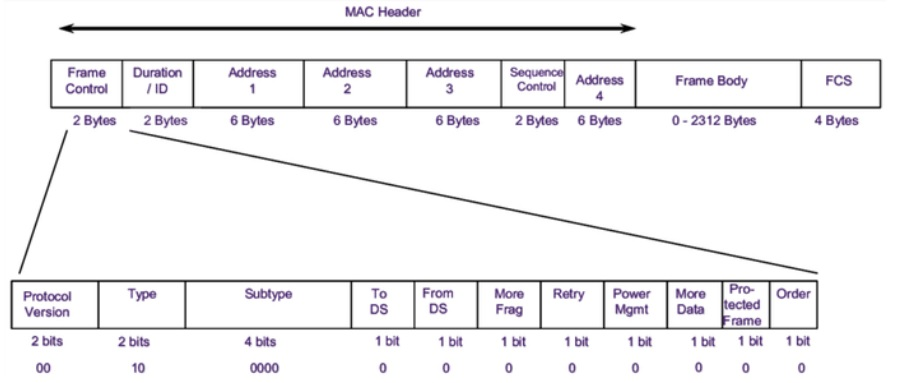
\includegraphics[width=0.8\textwidth]{img/OB-13_0.jpg}
	
	\item 4 různé MAC adresy s různými rolemi podle typu rámce:
	
	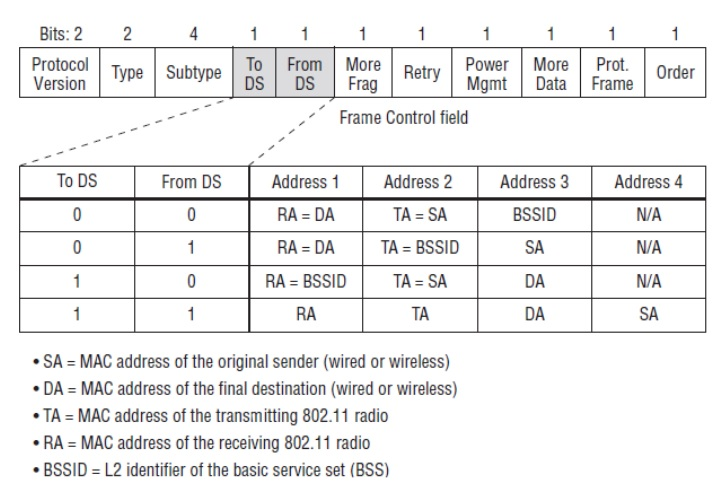
\includegraphics[width=0.8\textwidth]{img/OB-13_1.jpg}
	
	\item druhy rámců: management, control (RTS/CTS --- request to send, clear to send --- pro kontrolu toku dat), data
	
	\item management rámce
	\begin{itemize}
		\item Association request/response (žádost o připojení / odpověď)
		\item Reassociation request/response (znovupřipojení)
		\item Probe request/response (vyhledávání sítí, buď konkrétního SSID nebo všech)
		\item Beacon (ohlašování se --- vysílá se v pravidelných intervalech z AP, oznamuje jaké SSID jsou dostupná, spolu s konfigurací sítě)
		\item Authentication (proces pro ověření, zda je stanice schopna se připojit)
		\item Disassociation (bez odpovědi --- oznámení o odpojení)
		\item Deauthentication (resetuje stav připojení stanice)
		\item Action (vyvolají nějakou akci, lze pod to schovat nějaké nové typy rámců)
		\item Timing Advertisement (dnes se nepoužívá, předpokládáné využití v komunikaci se zařízeními co nemají vlastní čas)
	\end{itemize}
\end{itemize}

\subsubsection*{WEP}
\begin{itemize}
	\item Wired Eqivalent Privacy
	\item zastaralý bezpečnostní standard, vydán v roce 1999
	\item autentizace --- stanice pošle request, AP pošle v plaintextu challenge, stanice zašifruje a pošle reponse, dostane zpět potvrzení
	\item RC4 pro šifrování, CRC32 pro integritu
	
	\includegraphics[width=0.8\textwidth]{img/OB-13_2.jpg}
	
	\item problémy:
	\begin{itemize}
		\item sdílený klíč je používán pro autentizaci i pro šifrování dat
		\item znovupoužití keystreamu
		\item sdílený klíč se nemění (nebo jen málo často)
		\item IV se sdílí veřejně, je možné zachytit opakující se IV
		\item teoreticky 24 bitů IV, prakticky kolize po cca 5000 paketech
	\end{itemize}
\end{itemize}

\subsubsection*{WPA/WPA2}
\begin{itemize}
	\item Wi-Fi Protected Access
	\item různé módy autentizace --- personal (WPA-PSK, pre-shared key) nebo enterprise
	\item 4-way handshake (WPA/WPA2)
	
	\includegraphics[width=0.7\textwidth]{img/OB-13_3.jpg}
	
	\begin{itemize}
		\item PSK --- pre-shared key
		\item PMK --- pairwise master key = PBKDF2(HMAC-SHA1, PSK, SSID, 4096, 256) --- Password-Based Key Derivation Function 2
		\item PTK --- pairwise transit key = PRF(PMK, "Pairwise Key Expansion", MAC1, MAC2, nonce1, nonce2) --- Pseudo Random Function
		\item ANonce --- náhodné číslo AP
		\item SNonce --- náhodné číslo stanice
		\item případně GMK, GTK ---  Group Master/Temporal Key
	\end{itemize}
	\item problém s handshake --- lze zachytit a offline hádat klíč díky MIC --- Message Integrity Code spočítaný pomocí PTK
	\item šifrování v WPA --- TKIP (Temporal Key Integrity Protocol), založený na RC4
	\item šifrování v WPA2 --- CCMP (Ctr mode with CBC-MAC Protocol), založený na AES
\end{itemize}

\subsubsection*{WPA3}
\begin{itemize}
	\item obsahuje forward secrecy
	\item PMK se nevytváří z PSK
	\item vyřešený problém s handshake:
	
	\includegraphics[width=0.6\textwidth]{img/OB-13_4.jpg}
	
	\item SPEKE --- Simple Password Exponential Key Exchange
	\begin{itemize}
		\item A a B si dohodnou prvočíslo $p$, hash funkci $H$ a sdílené heslo $P$ (může být PSK u personal wifi)
		\item oba spočítají generátor $G = H(P)$
		\item následuje Diffie-Hellman výměna, spočítají společný klíč $K = |G^{a \cdot b}|_p$
	\end{itemize}
	\item existuje upravená verze "Dragonfly" využívající eliptických křivek
	\item stále lze na Wi-Fi útočit, lámat slabá hesla, zkoušt rainbow-tables pro nejznámější SSID, downgrade attack...
\end{itemize}
\subsection{OB-19 (HWB)}
Generátory skutečně náhodných čísel (TRNG), příklad konstrukce, základní vlastnosti. Srovnání s pseudo\-ná\-hod\-ný\-mi generátory (PRNG).


\subsubsection*{PRNG}
\begin{itemize}
	\item Pseudo Random Number Generator
	\item deterministické / algoritmické RNG
	\item má nějaký vnitřní stav a logiku přechodu do dalšího stavu, na základě stavu dává výstup
	\item výhoda je rychlost
	\item jeden z nejznámějších PRNG je lineární kongruenční generátor, definován rekurentním vztahem $X_{n + 1} = (a \cdot X_n + c)$ mod $m$, $X_0$ je počáteční hodnota zvaná seed
	\item $X$ se opakuje nejpozději po $m$ iteracích
	\item kvalita generátoru závisí na vybraných hodnotách $m, a, c$
	\item entropie musí být dodána dobrým seedem
	\item požadované bezpečnostní vlastnosti:
	\begin{itemize}
		\item  musí projít statistickými testy náhodnosti
		\item next-bit test --- na základě předchozích bitů nesmí být následující odhadnutelný
		\item "state compromise" / "backtracking resistance" --- z aktuálního vnitřního stavu generátoru nesmí jít zpětně rekonstruovat předchozí výstupy
	\end{itemize}
\end{itemize}

\subsubsection*{TRNG}
\begin{itemize}
	\item True Random Number Generator
	\item nedeterministický, nepředvídatelný
	\item typicky pomalejší a složitější než PRNG
	\item využívá jako zdroje entropie náhodné fyzikální či jiné procesy, které jsou složité předvídat
	\item horší statistické vlastnosti --- vhodné použít výstup jako seed do PRNG = hybridní RNG
	
	\item příklady: radioaktivní rozpad, teplotní šum, kvantové jevy, nestabilita oscilátoru, chování uživatele, parametry prostředí...
	\item nestabilita oscilátoru: 2 čítače se inkrementují podle 2 oscilátorů, a když jeden čítač dojde na požadovanou hodnotu, z hodnoty druhého se vezmou spodní bity --- náhodné
	\item TRNG založený na SRAM: SRAM po zapnutí napájení má náhodný obsah
	\item pro více bitů entropie lze pustit vícekrát
	\item jako postprocessing lze využít hashovací funkci, nebo např. Von Neumannův dekorelátor:
	
	\includegraphics[width=0.4\textwidth]{img/OB-19.jpg}
\end{itemize}
\subsection{OB-17 (HWB)}
Princip útoků postranními kanály. Typy postranních kanálů, časový útok na porovnání polí, útok jednoduchou odběrovou analýzou (SPA) na šifru RSA.

\subsubsection*{Princip}
\begin{itemize}
	\item typy útoků:
	\begin{itemize}
		\item invazivní / semi-invazivní / neinvazivní (z hlediska fyzického průniku)
		\item pasivní / aktivní (jen odposlech, nebo i manipulace s rozhraním)
	\end{itemize}
	\item útoky postranními kanály jsou typicky pasivní a neinvazivní
	\item postranní kanál je výměna informace mezi kryptografickým modulem a jeho okolím, není to součást jeho normální funkce ale spíš vedlejší příznak způsobený slabinou fyzické či softwarové implementace
	\item postranním kanálem lze obejít matematické principy, na kterých je založena bezpečnost kryptografických operací
	\item často dovolí odhadovat klíč po částech
	
	\includegraphics[width=0.5\textwidth]{img/OB-17_0.jpg}
\end{itemize}

\subsubsection*{Typy postraních kanálů}
\begin{itemize}
	\item časový postranní kanál --- doba vykonání operace závisí na tajemství, měřením času lze tajemství odhalit
	\item chybový postranní kanál --- chybový kód závisí na utajovaných datech
	\item odběrový postranní kanál (proudový / výkonový) ---  proudová spotřeba obvodu závisí na vnitřních datech v průběhu výpočtu šifry (simple/differential power analysis)
	\item elektromagnetický postranní kanál
	\item sociální kanál --- vyžaduje spolupráci uživatele
\end{itemize}

\subsubsection*{Časový útok na porovnání polí}
\begin{itemize}
	\item uvažujme 2 stejně velká pole, která chceme porovnat, dejme tomu zadané heslo vs správné heslo
	\item typicky porovnáváme po znacích/bytech, a když najdeme neshodu, končíme
	\item to je ale časový postranní kanál --- čím později porovnání skončí, tím více znaků od začátku je správně
	\item takto by správné heslo šlo hádat po znacích --- značně jednodušší než celé heslo naráz
	\item řešení: musí se vždy nějakým způsobem porovnat celé pole, tedy i když už víme že zadané heslo je špatné
\end{itemize}

\subsubsection*{Odběrový útok na RSA}
\begin{itemize}
	\item útok SPA --- Simple Power Analysis
	\item při dešifrování RSA dle vzorce $x = |c^d|_n$ se používá algoritmus Square and Multiply
	\item špatná implementace: square se provádí vždy (jednoduché, nízký odběr), a multiply se provádí jen  v případě, že aktuální bit je 1 (multiply je náročnější, vyšší odběr)
	\item v případě špatné implementace lze z odběru odhadnout, kdy se operace multiply prováděla a kdy ne, tedy sestavit bity tajné informace 
	
	\includegraphics[width=0.5\textwidth]{img/OB-17_1.jpg}
	
	\item správná implementace: multiply se provede vždy, pokud ale výsledek není potřeba tak se zahodí
\end{itemize}

\subsubsection*{DPA}
\begin{itemize}
	\item Differential Power Analysis
	\item mnoho průběhů, provádí se analýza signálu ve stejných okamžicích napříč všemi průběhy
	\item dále se předgenerují všechny možné hodnoty klíče, na základě toho také hypotetické spotřeby průběhů
	\item z hypotetických průběhů se najde ten, co nejvíce odpovídá reálným průběhům --- klíč odhalen
\end{itemize}
\subsection{OB-18 (HWB)}
Kontaktní a bezkontaktní čipové karty, princip činnosti a použití. Radiofrekvenční identifikace (RFID) a komunikace v blízkém poli (NFC).

\subsubsection*{Čipové karty obecně}
\begin{itemize}
	\item obvykle plastové kartičky obsahující integrovaný obvod
	\item obecněji --- nosič informace a bezpečnostních funkcí
	\item odolnost proti padělání
	\item lze použít např. pro vícefaktorovou autentizaci
	\item obsahuje vlastně počítač, který je: konfigurovatelný pomocí API, programovatelný při výrobě nebo i v térénu (java karty)
	\item z čeho se skládá: výpočetní jednotky (CPU, kryptografický koprocesor), paměti (RAM, ROM, EEPROM), komunikační zařízení, obvody napájení, senzory
\end{itemize}

\subsubsection*{Kontaktní karty}
\begin{itemize}
	\item rozhraní / konektor má typicky 6 nebo 8 pinů
	
	\includegraphics[width=0.4\textwidth]{img/OB-18_0.jpg}
	
	\item Inicializace připojení
	\begin{itemize}
		\item indikace přítomnosti karty
		\item zapnutí napájení
		\item signál hodin, reset
		\item karta pošle odpověď na reset (ATR --- Answer to Reset)
		\item dekódování ATR
		\item volba parametrů protokolu
	\end{itemize}
	\item přenos dat APDU (Application Protocol Data Unit --- něco jako aplikační vrstva) pomocí TPDU (Trans\-mission Protocol Data Unit --- něco jako transportní vrstva)
	\item T=0 --- byte oriented protocol
	\item T=1 --- block oriented protocol
\end{itemize}

\subsubsection*{Bezkontaktní karty}
\begin{itemize}
	\item zajímá nás hlavně norma ISO 14443 (vysoká frekvence --- 13.56MHz, komunikace na blízko), je používána často, jako v platebních kartách, lítačka, pas, průkaz ČVUT...
	\item RFID (RadioFrekvenční Identifikace)
	\begin{itemize}
		\item systém, který používá elektromagnetické pole k automatické identifikaci a sledování transponderů připevněných k objektům
		\item můžou se přenášet jak data tak napájení
		\item transponder --- nosič dat připevněný k objektu --- anténa + mikročip
		\item čtečka --- napájí a komunikuje s transpondery --- RF modul + řídící jednotka + anténa
	\end{itemize}
	\item NFC (Near FIeld Communication)
	\begin{itemize}
		\item rozšiřuje technologii RFID na bezdrátové datové rozhraní mezi zařízeními
		\item sada komunikačních protokolů pro přenos dat mezi dvěma zařízeními na krátkou vzdálenost (do cca 4 cm)
		\item pasivní transponder --- nemá baterii/zdroj napájení, všechna energie čerpána z čtečky
		\item aktivní transponder --- obsahuje baterii
		\item využití: bezkontaktní platební systémy, sdílení dat, elektronický průkaz, vstupní karta...
	\end{itemize}		 
\end{itemize}

\newpage
\section{Obecná bezpečnostní teorie}

\newpage
\section{Matematika}

\newpage
\section{Programování}

\end{document}
